\documentclass[11pt,a4paper]{article}
\usepackage[margin=25mm]{geometry}
\usepackage{amsmath,amssymb,amsthm,mathtools,mathrsfs,booktabs,graphicx,hyperref,xurl,microtype}
\hypersetup{hypertexnames=false,colorlinks=true,linkcolor=blue,urlcolor=blue}
\emergencystretch=2em
\providecommand{\tightlist}{\setlength{\itemsep}{0pt}\setlength{\parskip}{0pt}}
\title{Original Zeta, Full Support, and the Arithmetic Trace\\Exact heat, divisor and matrix reconstruction}
\author{Split-Zero research programme}
\date{23 September 2026}
\begin{document}
\maketitle
This continuation keeps the original Riemann zeta function and every
factor in its comparison with the theta heat family. It reconstructs
the exceptional local fibres, the full signed divisor and its finite
matrix receivers. In particular a calculated negative value of the
uncompensated full divisor is accompanied by its calculated positive
multiplier contribution. These different forms are related by the
proved formulas; no RH proof or disproof is asserted.
The full support lattice and all its prime stalks are derived
first. A faithful labelled heat source then gives a bounded
supported-zero action on its exact graph completion. Its two
prime-boundary moments evaluate as explicit theta values and
return the original zeta function. The final section constructs
both sectorial continuations of the unfiltered endpoint and
calculates the exact boundary direction lost by the theta filter.

\begin{figure}[htbp]
\centering
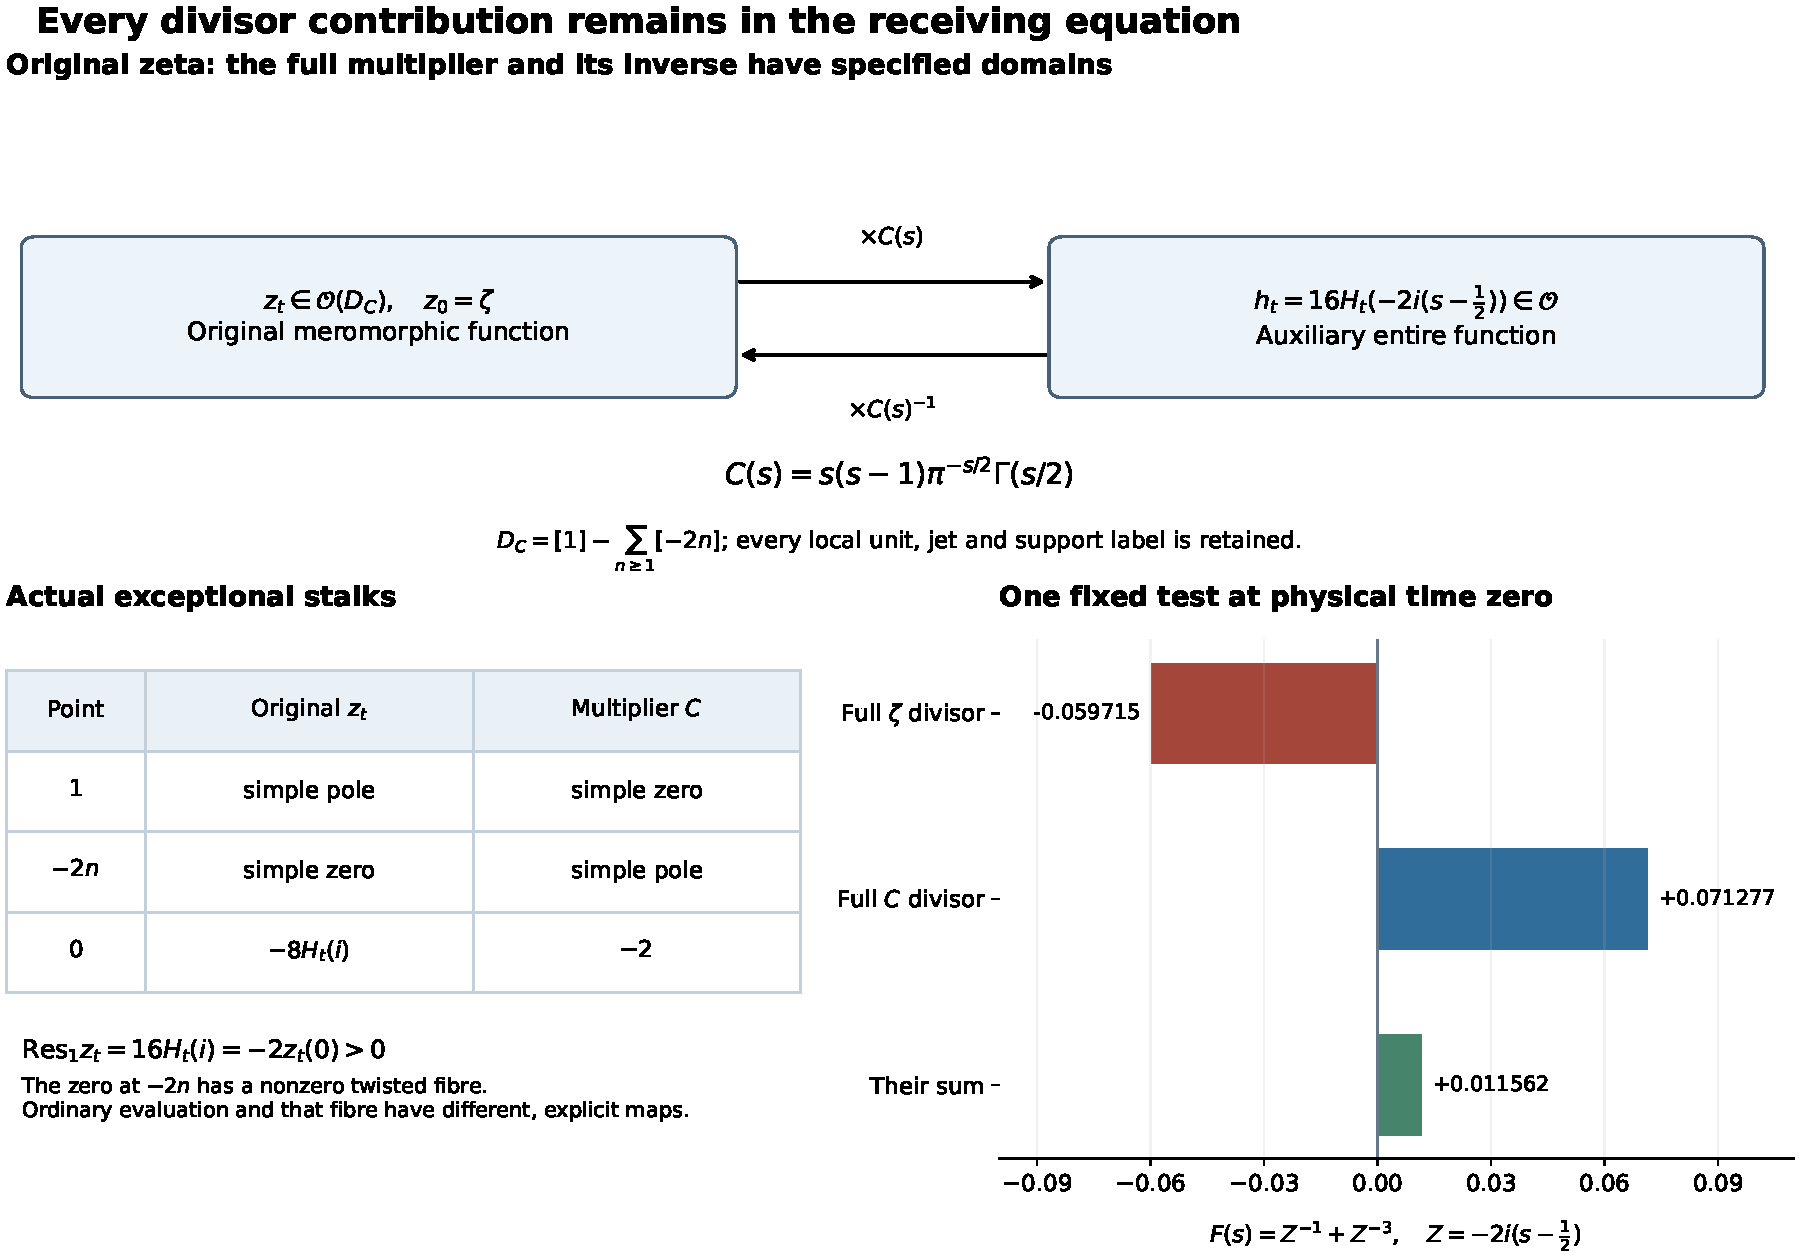
\includegraphics[width=\linewidth]{ORIGINAL_ZETA_RECEIVERS.pdf}
\caption{The actual multiplier and its line-module inverse (CF21),
all exceptional real stalks (CF16, CF27--28), and a fixed original
test at time zero (OZ8--13). Bar endpoints display midpoints of
certified intervals; the outward bounds and all tails are in the
proof. The heat source and constants are those of Rodgers--Tao,
arXiv:1801.05914v5, equations \texttt{htdef}, \texttt{hoz} and
\texttt{sas}. The two signed contributions are retained separately.}
\end{figure}
\clearpage
\tableofcontents
\section{Full-lattice primes, stalks, and retained factor
divisors}\label{full-lattice-primes-stalks-and-retained-factor-divisors}

Independent derivation, 2026-09-23. The actual bounded distributive
support lattice is retained throughout. No location claim about zeta
zeros follows from the spectrum alone.

\subsection{Original sources read}\label{original-sources-read}

The original
\href{https://github.com/KokunoYumeto/zeta-function-research-reader/blob/d2f0020a7c446f429682925c1c682d99ba86a4cc/workbenches/splitzero-tandem/foundations/globalization-semiring/globalization_note.tex}{globalization
note} supplies the two-label construction. Its relevant labels and
source lines are thm:ideal-classification (207), cor:prime-ideals (239),
cor:dim-two (262), thm:zero-prime-not-irr (298),
thm:localization-away-from-zero (436), thm:frac-collapse (482), and
cor:stalks (534).

The original
\href{https://github.com/KokunoYumeto/zeta-function-research-reader/blob/a2851f9eb352e7e4376bc629de86fa4ed9c1c434/workbenches/splitzero-tandem/foundations/split-support-geometry-v11/split_support_geometry_arithmetic_curve_v11.tex}{full-lattice
geometry, version 11} supplies the lattice construction. Its locators
are def:lattice-split (1229--1252), thm:lattice-normal-form
(1255--1308), thm:lattice-localization (1457--1489),
thm:lattice-ideal-classification (1619--1658),
thm:lattice-prime-classification (1662--1701), thm:spectral-ordinal-sum
(1710--1747), cor:lattice-split-dimension (1750--1769), branch
construction (1877--1925), and thm:branch-selected-spectrum
(1929--1973). The arithmetic retraction is at prop:classical-collapse
(4653--4675), and the vector support construction at
prop:split-anomaly-line (7573--7602).

The required algebra is fully proved below. These citations identify the
original versions and exact source sections used; the results are
rederived on the full lattice.

\subsection{LP1. The actual semiring and universal
maps}\label{lp1.-the-actual-semiring-and-universal-maps}

Let \(R\) be a nonzero commutative unital ring and \(L\) a nontrivial
bounded distributive lattice, with bottom \(0_L\), top \(1_L\), join
\(\vee\), and meet \(\wedge\). Set \[
S=G_L(R)=\{(0,\lambda):\lambda\in L\}\cup\{(r,1_L):r\in R\},
\tag{LP1.1}
\] \[
(r,\lambda)+(s,\mu)=(r+s,\lambda\vee\mu),\qquad
(r,\lambda)(s,\mu)=(rs,\lambda\wedge\mu).
\tag{LP1.2}
\] Write \(z_\lambda=(0,\lambda)\), \(\tau=z_{0_L}\), \(e=z_{1_L}\), and
\(\widetilde r=(r,1_L)\). Thus \(\widetilde0=e\ne\tau\). A nonzero
amplitude requires top support. Closure holds because a nonzero sum has
a top-support summand and a nonzero product has two top-support factors.
Associativity and commutativity are componentwise, and distributivity is
the ring and lattice distributive laws. The additive identity is
\(\tau\), and the multiplicative unit is \(\widetilde1\).

Both projections are semiring maps: \[
p_L:S\to R,\quad(r,\lambda)\mapsto r,\qquad
\chi_L:S\to L,\quad(r,\lambda)\mapsto\lambda.
\tag{LP1.3}
\] Put \(Z_L=\{z_\lambda:\lambda\in L\}\). Every semiring map from \(S\)
to a ring kills \(Z_L\), because \(e+z_\lambda=e\) and additive
cancellation in the target force the image of \(z_\lambda\) to be zero.
Its restriction to the supported \(R\) is then a unital ring map.
Conversely every such ring map extends by killing \(Z_L\). This proves
the universal property of \(p_L\).

The units are exactly \(\widetilde u\), \(u\in R^\times\): equality of a
product with \(\widetilde1\) forces the amplitudes to multiply to \(1\);
conversely the ring inverse at top support is a semiring inverse. In
particular \(e\) is a nonunit.

\subsection{LP2. All ideals, all primes, and their
order}\label{lp2.-all-ideals-all-primes-and-their-order}

For a proper lattice ideal \(\mathfrak a\) and ring ideal \(J\), define
\[
Z_{\mathfrak a}=\{z_\lambda:\lambda\in\mathfrak a\},\qquad
I_J=Z_L\cup\{\widetilde r:r\in J\}.
\tag{LP2.1}
\] A lattice ideal contains bottom, is lower, and is closed under finite
joins. Every semiring ideal has exactly one of these forms. If it
contains \(\widetilde r\), multiplication by \(\widetilde{-1}\) and
addition put \(e\) in it, and \(ez_\lambda=z_\lambda\) puts all of
\(Z_L\) in it. Its top-support amplitudes form a ring ideal by addition
and scalar absorption. If it contains no top-support element, it lies in
\(Z_L\) and omits \(e\). Its labels are join-closed, and
\(\mu\le\lambda\) gives \(z_\mu=z_\mu z_\lambda\), proving lower
closure. Conversely the displayed sets are ideals by LP1.2. Their
parameters are uniquely recovered, and the families are disjoint because
only the second contains \(e\).

A lattice prime is a proper lattice ideal for which membership of
\(\lambda\wedge\mu\) implies membership of one factor. The prime ideals
of \(S\) are exactly \[
P_{\mathfrak p}=Z_{\mathfrak p}\quad
(\mathfrak p\in\operatorname{Spec}_{\rm lat}L),\qquad
Q_{\mathfrak q}=I_{\mathfrak q}\quad
(\mathfrak q\in\operatorname{Spec}R).
\tag{LP2.2}
\] For a support ideal, two top-support factors have top-support product
even when its amplitude vanishes. A zero-fiber factor multiplied by top
support remains that factor. Two zero-fiber factors multiply by meet.
These three cases prove exactly lattice primality. For an amplitude
ideal, a product with a zero-fiber factor already has a factor in the
ideal; top-support products give exactly ring primality. LP2.1 proves
exhaustion.

The full order is \[
\begin{aligned}
P_{\mathfrak p}\subseteq P_{\mathfrak p'}&\iff\mathfrak p\subseteq\mathfrak p',\\
Q_{\mathfrak q}\subseteq Q_{\mathfrak q'}&\iff\mathfrak q\subseteq\mathfrak q',\\
P_{\mathfrak p}&\subsetneq Q_{\mathfrak q}\quad\text{for all }\mathfrak p,\mathfrak q.
\end{aligned}\tag{LP2.3}
\] Read labels and amplitudes for the first two statements. The last is
strict because the amplitude prime contains \(e\).

\subsection{LP3. Supported-zero principal prime and
dimension}\label{lp3.-supported-zero-principal-prime-and-dimension}

Multiplication and join closure give \[
(z_\lambda)=z_\lambda S=\{z_\mu:\mu\le\lambda\},\qquad
(e)=Z_L.
\tag{LP3.1}
\] Thus \[
(e)\text{ is prime}\iff R\text{ is an integral domain}.
\tag{LP3.2}
\] For a domain, divisibility by \(e\) is membership in this prime
ideal, so \(e\mid ab\) forces \(e\mid a\) or \(e\mid b\). But \(e=e^2\)
factors into two nonunits, so \(e\) is not irreducible. For
\(\lambda<1_L\), \((z_\lambda)\) is prime exactly when
\(\downarrow\lambda\) is a prime lattice ideal. In particular \((\tau)\)
is prime exactly when bottom is meet-prime, which fails for two disjoint
nonempty masks in a power-set lattice.

Write \(h=\dim\operatorname{Spec}_{\rm lat}L\), defined as the supremum
of finite strict chain lengths, possibly infinite. This spectrum is
nonempty under the usual axiom of choice. Indeed Zorn gives a maximal
proper lattice ideal. If \(a\wedge b\) belongs to it but neither \(a\)
nor \(b\) does, maximality supplies \(u,v\) in it with
\(u\vee a=v\vee b=1_L\). Distributivity gives \[
1_L=(u\vee a)\wedge(v\vee b)\le u\vee v\vee(a\wedge b),
\] contradicting properness. Hence that ideal is prime.

For a domain \(R\), \[
\operatorname{ht}_S(e)=h+1,\quad
\operatorname{ht}_S Q_{\mathfrak q}=h+1+\operatorname{ht}_R\mathfrak q,\quad
\dim S=h+1+\dim R.
\tag{LP3.3}
\] Each finite prime chain is a support chain followed by an amplitude
chain, with one possible transition. Conversely every two chosen finite
chains concatenate with one strict transition. Below \(Q_{(0)}\) the
amplitude part consists only of that point. Taking suprema proves every
formula, including infinite values. For \(R=\mathbb Z\), the dimension
is \(h+2\). For \(L=C_n=\{0<1<\cdots<n\}\), its \(n\) proper nonempty
initial segments are exactly its prime ideals, and form a chain of
length \(n-1\). Therefore \[
\dim G_{C_n}(\mathbb Z)=n+1,\qquad \operatorname{ht}(e)=n.
\tag{LP3.4}
\] This gives arbitrarily large height for the principal supported-zero
prime while preserving the arithmetic coefficient ring.

\subsection{LP4. Arithmetic closed
stratum}\label{lp4.-arithmetic-closed-stratum}

Prime membership gives \[
D_S(z_\lambda)=\{P_{\mathfrak p}:\lambda\notin\mathfrak p\},\qquad
D_S(\widetilde r)=\operatorname{Spec}_{\rm lat}L\cup D_R(r).
\tag{LP4.1}
\] These basic opens prove the ordinal-sum topology and \[
D_S(e)=\operatorname{Spec}_{\rm lat}L,\qquad
V_S(e)=\{Q_{\mathfrak q}:\mathfrak q\in\operatorname{Spec}R\}.
\tag{LP4.2}
\] The reflection induces the closed embedding \[
i:\operatorname{Spec}R\to\operatorname{Spec}S,\quad
\mathfrak q\mapsto Q_{\mathfrak q}.
\tag{LP4.3}
\] The quotient congruence is exactly equality of amplitudes: the Bourne
relation \(x+a=y+b\), \(a,b\in Z_L\), implies equal amplitudes;
conversely equal amplitudes give \(x+e=y+e\). Hence this quotient is
\(R\).

For a domain there is a topological retraction \[
r(P_{\mathfrak p})=(0),\qquad r(Q_{\mathfrak q})=\mathfrak q,\qquad ri=\mathrm{id}.
\tag{LP4.4}
\] The inverse image of \(D_R(a)\) for \(a\ne0\) is
\(D_S(\widetilde a)\); that of \(D_R(0)\) is empty. This proves
continuity. The closure of \((e)\) is precisely the arithmetic closed
stratum.

This retraction cannot lift to a unital semiringed-space retraction: its
map at \(Q_{(0)}\) would require a unital semiring map \(K\to G_L(K)\),
where \(K=\operatorname{Frac}R\). Composing any such map with \(\chi_L\)
and applying it to \(1+(-1)=0\) gives \(1_L\vee\lambda=0_L\),
impossible. The exact surviving bridges are the quotient embedding LP4.3
with its stalk maps below, and the proved topological retraction LP4.4.

\subsection{LP5. All prime stalks with full
lattice}\label{lp5.-all-prime-stalks-with-full-lattice}

Semiring fractions satisfy \[
(a,s)\sim(b,t)\iff\exists u\text{ in the denominators}:uat=ubs.
\tag{LP5.1}
\] The complement of \(Q_{\mathfrak q}\) consists of \(\widetilde s\),
\(s\notin\mathfrak q\). There is an isomorphism \[
S_{Q_{\mathfrak q}}\longrightarrow G_L(R_{\mathfrak q}),\quad
\frac{(a,\lambda)}{\widetilde s}\mapsto(a/s,\lambda).
\tag{LP5.2}
\] It preserves operations, is onto, and equality in the target means
equal labels and \(u(at-bs)=0\) for some \(u\notin\mathfrak q\). These
are precisely LP5.1, proving injectivity and well-definedness. If a
nonzero numerator becomes zero in the localized ring, it retains its top
label and becomes \(e\).

For a domain this yields \[
\boxed{S_{(e)}\cong G_L(\operatorname{Frac}R).}
\tag{LP5.3}
\] Every lattice label survives. By contrast, \[
\boxed{S[e^{-1}]\cong L.}
\tag{LP5.4}
\] An invertible idempotent is the unit, so any map inverting \(e\)
identifies \(x\) with \(ex=z_{\chi_L(x)}\) and factors uniquely through
\(\chi_L\), which itself inverts \(e\). The same argument gives
\(S[z_\lambda^{-1}]\cong\downarrow\lambda\), using LP3.1 and the
idempotent \(z_\lambda\) as the new unit.

At \(P_{\mathfrak p}\), \(e\) belongs to the denominator set. First
apply LP5.4, then invert \(F=L\setminus\mathfrak p\): \[
\boxed{S_{P_{\mathfrak p}}\cong L_{\mathfrak p}=F^{-1}L.}
\tag{LP5.5}
\] Every fraction is represented by a label, with exact equivalence \[
\lambda\equiv_{\mathfrak p}\mu
\iff\exists f\in F:\lambda\wedge f=\mu\wedge f.
\tag{LP5.6}
\] Every inverted idempotent becomes \(1\). The displayed relation is
reflexive with witness \(1_L\), symmetric, transitive using the meet of
witnesses, and compatible with join and meet by distributivity. It
identifies every \(f\in F\) with \(1_L\); any map doing this respects
the displayed relation. This proves its universal property.

A class equals \(1\) exactly when its label is outside \(\mathfrak p\):
use the label itself as witness in one direction; in the other,
\(\lambda\wedge f=f\) with \(\lambda\in\mathfrak p,f\in F\) contradicts
lower closure. The quotient remains a lattice and has only one unit, its
top, because \(x\wedge y=1\) forces \(x=y=1\). Its unique maximal ideal
is the image of \(\mathfrak p\).

For finite \(L\), put \(f_{\mathfrak p}=\bigwedge F\in F\). Then \[
L_{\mathfrak p}\cong\downarrow f_{\mathfrak p},\quad
[\lambda]\mapsto\lambda\wedge f_{\mathfrak p}.
\tag{LP5.7}
\] Equality after meet with a witness \(f\in F\) implies equality after
meet with \(f_{\mathfrak p}\le f\), and the converse uses
\(f_{\mathfrak p}\). Every label below \(f_{\mathfrak p}\) occurs. For
\(L=\{0<a<1\}\), the prime \(\{0,a\}\) has stalk all of \(L\), since its
complement is \(\{1\}\). Thus support stalks are not generally Boolean.

\subsection{LP6. Stalk arrows and explicit
branches}\label{lp6.-stalk-arrows-and-explicit-branches}

At the arithmetic closed stratum, the local reflection is \[
G_L(R_{\mathfrak q})\to R_{\mathfrak q},\quad(a,\lambda)\mapsto a.
\tag{LP6.1}
\] It is local because its inverse image of ring units is precisely the
units identified in LP1. Its zero fiber is the complete \(L\). The
contravariant maps along every prime inclusion are \[
\begin{array}{ll}
Q_{\mathfrak q}\subseteq Q_{\mathfrak q'}:
&G_L(R_{\mathfrak q'})\to G_L(R_{\mathfrak q}),\quad(a/s,\lambda)\mapsto(a/s,\lambda),\\
P_{\mathfrak p}\subseteq P_{\mathfrak p'}:
&L_{\mathfrak p'}\to L_{\mathfrak p},\quad[\lambda]_{\mathfrak p'}\mapsto[\lambda]_{\mathfrak p},\\
P_{\mathfrak p}\subsetneq Q_{\mathfrak q}:
&G_L(R_{\mathfrak q})\to L_{\mathfrak p},\quad(a,\lambda)\mapsto[\lambda]_{\mathfrak p}.
\end{array}\tag{LP6.2}
\] The first two increase denominator sets. The last is support
projection followed by LP5.6, and every arithmetic denominator maps to
the unit. Thus each is the exact localization map; all triangles
commute.

An explicit bounded lattice homomorphism \(\epsilon:L\to\mathbf B\), and
only such a selected branch in this construction, gives \[
\beta_\epsilon:G_L(R)\to G_{\mathbf B}(R),\quad
z_\lambda\mapsto z_{\epsilon(\lambda)},\quad\widetilde r\mapsto\widetilde r.
\tag{LP6.3}
\] Join and meet preservation prove the homomorphism. Taking preimages
of the primes in LP2.2 shows that its spectral image is the selected
\(P_{\epsilon^{-1}(0)}\) together with all \(Q_{\mathfrak q}\). No
branch was selected in the preceding results.

\subsection{LP7. Analytic local rings and full meromorphic
germs}\label{lp7.-analytic-local-rings-and-full-meromorphic-germs}

Let \(Y\) be a nonsingular connected complex curve, \(y\in Y\),
\(\mathcal O_y\) its holomorphic local ring, \(\mathfrak m_y\) its
maximal ideal, and \(\mathcal M_y=\operatorname{Frac}\mathcal O_y\). The
integral coefficient map induces \[
G_L(\mathbb Z)\to G_L(\mathcal O_y),\quad(n,\lambda)\mapsto(n\cdot1,\lambda).
\tag{LP7.1}
\] It preserves every label and commutes with amplitude reflection.

For a chosen local parameter \(w\) at \(y\), the first nonzero Taylor
coefficient gives the exact full factorization \[
f=w^n u,\qquad n\ge0,\quad u\in\mathcal O_y^\times
\tag{LP7.2}
\] for every nonzero holomorphic germ. Quotients give the same
expression for meromorphic germs with \(n\in\mathbb Z\). The entire unit
\(u\) is retained. A new parameter \(w'=wv\), \(v\) a unit, gives
\(u'=v^{-n}u\); this proves \(n\) is intrinsic and proves the full
change formula. Multiplication adds \(n\) and multiplies the full units.
Hence \[
1\to\mathcal O_y^\times\to\mathcal M_y^\times
\xrightarrow{\operatorname{ord}_y}\mathbb Z\to0
\tag{LP7.3}
\] is exact: its kernel is the retained unit group, and \(w^n\) attains
each integer. The original germs are kept in the source; the order image
does not replace them.

A nonzero ideal of \(\mathcal O_y\) has a least order \(n\); an element
of that order is \(w^n\) times a unit, so the ideal is \((w^n)\). Thus
its only nonzero prime is \(\mathfrak m_y=(w)\). The full lattice prime
chain and its arithmetic stalks are \[
P_{\mathfrak p}\subsetneq Q_{(0)}=(e)\subsetneq Q_{\mathfrak m_y},
\tag{LP7.4}
\] \[
\bigl(G_L(\mathcal O_y)\bigr)_{Q_{(0)}}=G_L(\mathcal M_y),\qquad
\bigl(G_L(\mathcal O_y)\bigr)_{Q_{\mathfrak m_y}}=G_L(\mathcal O_y).
\tag{LP7.5}
\] Here equality denotes the explicit isomorphisms LP5.2. Evaluation \[
G_L(\mathcal O_y)\to G_L(\mathbb C),\quad(f,\lambda)\mapsto(f(y),\lambda)
\tag{LP7.6}
\] has amplitude-zero inverse image \(Q_{\mathfrak m_y}\). A nonzero
germ vanishing at \(y\) evaluates to \(e\), with top support; before
evaluation LP7.2 retains its exact order and full unit. A pole is a
meromorphic germ with negative order. The element \(e\) is not a
parameter: \(e^2=e\). Equations LP7.3--LP7.6 give its precise relation
to meromorphic localization and analytic orders.

\subsection{LP8. Full factor source and tagged divisor
module}\label{lp8.-full-factor-source-and-tagged-divisor-module}

Let \(\mathcal A\) be a nonempty finite set of original factor labels
and let \(F_\alpha\), \(\alpha\in\mathcal A\), be specified nonzero
meromorphic functions on \(Y\). Every original constant, power, and
factor remains in this tuple, including factors with zero divisor. Put
\[
D=\bigcup_{\alpha\in\mathcal A}
\{y:\operatorname{ord}_yF_\alpha\ne0\}.
\tag{LP8.1}
\] The set is locally finite by isolation of zeros and poles and
finiteness of \(\mathcal A\). Points at which the product has net order
zero are retained. At every \(y\in Y\), including outside \(D\), the
entire original germ tuple in \((\mathcal M_y^\times)^{\mathcal A}\)
remains available.

With \(S_{\mathbb Z}=G_L(\mathbb Z)\), define \[
\mathscr T_L(U)=\prod_{y\in D\cap U}S_{\mathbb Z}^{\mathcal A},\qquad
\mathscr C_L(U)=\prod_{y\in D\cap U}S_{\mathbb Z}.
\tag{LP8.2}
\] Restrictions delete coordinates outside a smaller open.
Coordinatewise operations make these sheaves of semimodules: compatible
sections glue uniquely at each coordinate. Their stalks at \(y\in D\)
are \(S_{\mathbb Z}^{\mathcal A}\), \(S_{\mathbb Z}\), since a
sufficiently small neighborhood contains no other divisor point; away
from \(D\) the stalk is zero. Products allow globally infinite divisors
without dropping their locally finite contributions.

Define integral amplitude sheaves \[
\mathscr D_{\rm tag}(U)=\prod_{y\in D\cap U}\mathbb Z^{\mathcal A},\qquad
\mathscr D(U)=\prod_{y\in D\cap U}\mathbb Z.
\tag{LP8.3}
\] Amplitude and support give an injection \[
\mathscr T_L(U)\hookrightarrow
\mathscr D_{\rm tag}(U)\times\prod_{y\in D\cap U}L^{\mathcal A}.
\tag{LP8.4}
\] Its image is exactly the pairs satisfying
\(n_{\alpha,y}\ne0\Rightarrow\lambda_{\alpha,y}=1_L\). This is LP1.1
coordinatewise; in particular the amplitude-zero fiber is the entire
product of lattice labels.

The supplied factor tuple maps to \[
(\mathbf d_F)_{\alpha,y}=(\operatorname{ord}_yF_\alpha,1_L).
\tag{LP8.5}
\] Every supplied factor has an entry at every point of \(D\). An
order-zero factor has value \(e\), not absence. The complete functions
and unit germs are retained separately in the source tuple. The exact
local map is \[
\begin{array}{ccc}
(\mathcal M_y^\times)^{\mathcal A}&\xrightarrow{\prod_\alpha}&\mathcal M_y^\times\\
\downarrow(\operatorname{ord}_y)_\alpha&&\downarrow\operatorname{ord}_y\\
\mathbb Z^{\mathcal A}&\xrightarrow{\sum_\alpha}&\mathbb Z.
\end{array}\tag{LP8.6}
\] Both vertical maps are onto, with kernels
\((\mathcal O_y^\times)^{\mathcal A}\) and \(\mathcal O_y^\times\), by
LP7.3. The square commutes because orders add. It specifies the
information carried by the divisor image and the full unit information
remaining in the source. The supplied top-support lift of an order tuple
is not claimed to preserve additive zero: a supplied zero order
intentionally maps to \(e\).

\subsection{LP9. Exact cancellation and supported
fibers}\label{lp9.-exact-cancellation-and-supported-fibers}

Finite tag sum is the semimodule map \[
\Delta:\mathscr T_L\to\mathscr C_L,\quad
((n_\alpha,\lambda_\alpha))_\alpha\mapsto
\left(\sum_\alpha n_\alpha,\bigvee_\alpha\lambda_\alpha\right).
\tag{LP9.1}
\] Additivity follows from associativity and commutativity. Scalar
compatibility follows from integer distributivity and
\(\bigvee_\alpha(\mu\wedge\lambda_\alpha)=\mu\wedge\bigvee_\alpha\lambda_\alpha\).
Thus \(\Delta\) is \(S_{\mathbb Z}\)-linear. It is onto by putting a
target in one tag and \(\tau\) in all others. The amplitude square with
the ordinary sum \(\Sigma:\mathscr D_{\rm tag}\to\mathscr D\) commutes
coordinatewise. For the supplied tuple, \[
\Delta(\mathbf d_F)_y=
\left(\operatorname{ord}_y\prod_\alpha F_\alpha,1_L\right).
\tag{LP9.2}
\] Cancellation gives \(e\ne\tau\), while every original factor order
remains in \(\mathbf d_F\) and every full factor remains in LP8.6.

The exact fibers at a divisor point are \[
\begin{aligned}
\Delta^{-1}(e)&=\{(n_\alpha,\lambda_\alpha):
\sum_\alpha n_\alpha=0,\ \bigvee_\alpha\lambda_\alpha=1_L\},\\
\Delta^{-1}(\tau)&=\{(\tau)_\alpha\}.
\end{aligned}\tag{LP9.3}
\] The first is equality of the two output coordinates. For the second,
a finite join equals bottom only when all entries are bottom, and each
bottom label forces amplitude zero. The full congruence is equality of
the sums and equality of the joins; it is not determined merely by the
additive-zero preimage.

For \(k=|\mathcal A|\), the canceled integer subgroup has the complete
split exact sequence \[
0\to\mathbb Z^{k-1}
\xrightarrow{(a_1,\ldots,a_{k-1})\mapsto
(a_1,\ldots,a_{k-1},-\sum_{j<k}a_j)}
\mathbb Z^k\xrightarrow{\Sigma}\mathbb Z\to0.
\tag{LP9.4}
\] The first map is injective with exactly the zero-sum image, and the
last is split by its last coordinate. For \(k=1\) the first group is
zero. This identifies the canceled integer data and relates them to the
supported fiber without deleting the tags.

\subsection{LP10. Tagged source at the actual coefficient
primes}\label{lp10.-tagged-source-at-the-actual-coefficient-primes}

At \(y\in D\), the fiber is finite free. For every coefficient prime
\(P\), \[
(S_{\mathbb Z}^{\mathcal A})_P\cong(S_{\mathbb Z,P})^{\mathcal A}.
\tag{LP10.1}
\] The map is coordinatewise. Multiply the finitely many denominators to
get a common denominator for surjectivity, and multiply the finitely
many equality witnesses from LP5.1 for injectivity. No commutation with
an infinite product of global sections is asserted. Thus the three kinds
of fibers are \[
\begin{array}{ll}
P=(e):&G_L(\mathbb Q)^{\mathcal A},\\
P=Q_{(p)}:&G_L(\mathbb Z_{(p)})^{\mathcal A},\\
P=P_{\mathfrak p}:&L_{\mathfrak p}^{\mathcal A}.
\end{array}\tag{LP10.2}
\] The tag-sum map commutes with localization by linearity. The maps
from \(G_L(\mathbb Z)\) to \(G_L(\mathbb Q)\) and
\(G_L(\mathbb Z_{(p)})\) are injective, because both preserve labels and
their ring maps reflect equality of integers. Consequently every tagged
signed integer order and every canceled integer vector survives at the
supported-zero and arithmetic prime stalks, and \(e\) remains distinct
from \(\tau\).

At a support prime the exact map is
\((n,\lambda)\mapsto[\lambda]_{\mathfrak p}\). Each supplied top-support
order becomes top independently in each tag. This is the exact support
image; the original factor source and arithmetic stalks retain the
integer and germ data through the proved maps.

\subsection{LP11. Scope for original
zeta}\label{lp11.-scope-for-original-zeta}

The base contributes the full meromorphic stalk at the supported-zero
prime, the arithmetic amplitude quotient, all support stalks, the local
valuation sequence with its retained unit kernel, and a tagged source
whose cancellation map sends zero sums to \(e\). These are exact maps
available to the original zeta and completion-factor calculations.

They do not alone force zero locations. For example, in the original
complex coordinate \(s\), translation gives \[
\mathcal O_{\mathbb C,y+a}\to\mathcal O_{\mathbb C,y},\quad F(s)\mapsto F(s+a).
\tag{LP11.1}
\] Its inverse is translation by \(-a\). It preserves maximal ideals,
extends to meromorphic fields, preserves each order and its full
transported unit, and induces \(G_L\)-isomorphisms fixing all labels.
Indeed \(s+a-(y+a)=s-y\), so the full local factorization transports
exactly. The tagged divisor point \(y+a\) maps to \(y\) with every
coefficient and factor label retained, and the cancellation square
commutes. This is a comparison of local structures, not a coordinate
substitution in an original zeta calculation. The actual original
functions, completion factors, symmetries and differential terms supply
the further analytic data.

The original-zeta trace and heat calculations receive this base through
the exact stalk and factor maps above. Their analytic functions and
differential terms remain additional specified data.

\section{The original zeta function with its complete meromorphic factor retained}
\label{sec:completion-factor-full-heat-map}

\paragraph{CF1. Original source, coordinates, and multiplier.}
The original author source is Brad Rodgers and Terence Tao,
\href{https://arxiv.org/abs/1801.05914v5}{\emph{The de Bruijn--Newman
constant is non-negative}}, version 5, equations
\texttt{hoz}, \texttt{sas}, \texttt{phidef}, and \texttt{htdef}.
The defining passage was read directly in its retained author
TeX, lines 75--106; no claim of a complete reading is made here.
It gives exactly
\[
 \begin{split}
 \Phi(u)&=\sum_{n=1}^{\infty}
 (2\pi^2n^4e^{9u}-3\pi n^2e^{5u})e^{-\pi n^2e^{4u}},\\
 H_t(Z)&=\int_0^\infty e^{tu^2}\Phi(u)\cos(Zu)\,du,\\
 H_0(Z)&=\frac18\xi\!\left(\frac12+\frac{iZ}{2}\right),
 \qquad
 \xi(s)=\frac{s(s-1)}2\pi^{-s/2}\Gamma(s/2)\zeta(s).
 \end{split}\tag{CF1}
\]
Here \(\zeta\) is the original Riemann zeta function, initially
\(\sum_{n\ge1}n^{-s}\) on \(\Re s>1\), with its meromorphic
continuation. Keep the precise receiving map
\[
 \begin{gathered}
 Z=-2i(s-\tfrac12),\qquad
 h_t(s)=16H_t\!\left(-2i(s-\tfrac12)\right),\\
 C(s)=s(s-1)\pi^{-s/2}\Gamma(s/2),\qquad
 h_0(s)=2\xi(s)=
 \underbrace{s(s-1)\pi^{-s/2}\Gamma(s/2)}_{C(s)}\zeta(s).
 \end{gathered}\tag{CF2}
\]
Every appearance of \(C\) below refers to this full meromorphic
function. None of its four displayed factors is discarded.

The Gamma input is the original-author treatment of Ricardo
P\'erez-Marco,
\href{https://arxiv.org/abs/2001.04445v2}{\emph{On the definition
of Euler Gamma function}}, version 2, Theorem
\texttt{thm:main-Euler-gamma}, Corollary \texttt{cor:W-product},
and Corollary \texttt{cor:Gamma(1/2)}. Its original TeX
\path{definition-gamma-Euler6.tex} and intact source archive
are retained. The direct reading covers lines 202--340,
1170--1205, and the Euler-integral theorem at 1332--1389.
We also use the primary TeX equations in R.\ A.\ Askey and
R.\ Roy's \href{https://dlmf.nist.gov/5}{DLMF Chapter 5}:
\href{https://dlmf.nist.gov/5.5.E1}{5.5.1},
\href{https://dlmf.nist.gov/5.7.E3}{5.7.3},
\href{https://dlmf.nist.gov/5.7.E4}{5.7.4}, and
\href{https://dlmf.nist.gov/5.8.E2}{5.8.2}.
All four equation TeX files are retained and were read completely.
Their required consequences are derived below.

\paragraph{CF2. Analyticity, positivity, and the exact heat clock.}
Every summand of \(\Phi(u)\) is strictly positive for \(u\ge0\):
its sign is the sign of \(2\pi n^2e^{4u}-3>0\).
There is a finite constant \(K_\Phi>0\) such that
\[
 0<\Phi(u)\le K_\Phi e^{9u}e^{-\pi e^{4u}/2},
 \qquad u\ge0.
 \tag{CF3}
\]
Indeed, each complete summand is at most
\(2\pi^2n^4e^{9u}e^{-\pi n^2e^{4u}}\).
For \(E=e^{4u}\ge1\),
\(n^2E\ge E/2+n^2/2\), so
\[
 \sum_{n\ge1}n^4e^{-\pi n^2E}
 \le e^{-\pi E/2}\sum_{n\ge1}n^4e^{-\pi n^2/2}.
\]
This proves CF3 with
\(K_\Phi=2\pi^2\sum_{n\ge1}n^4e^{-\pi n^2/2}\).
It does not change the kernel in CF1.

On a compact set of complex \(t,Z\), every mixed derivative
of the integrand is bounded by a constant times
\[
 u^N\exp(Tu^2+Bu+9u-\pi e^{4u}/2)
\]
for some finite \(N,T,B\). This is integrable: \(e^{4u}\)
eventually dominates every polynomial in \(u\), and the
integrand is bounded on finite intervals. Differentiation
under the integral and locally uniform convergence therefore
prove joint entire dependence on \(t,Z\), and
\[
 \partial_tH_t=-\partial_Z^2H_t.
\]
Since \((-2i)^2=-4\), applying the actual map CF2 gives
\[
 \partial_t h_t(s)=\frac14\partial_s^2h_t(s).
 \tag{CF4}
\]
The factor \(1/4\) is forced by the original arithmetic
coordinate and is not a choice of heat clock.

For real \(t,y\), the complete integral is
\[
 H_t(iy)=\int_0^\infty e^{tu^2}\Phi(u)\cosh(yu)\,du>0.
 \tag{CF5}
\]
Evenness of the cosine gives \(h_t(1-s)=h_t(s)\), including
complex \(s,t\). In particular, for every real \(t,s\),
\(h_t(s)>0\). None of the real exceptional points examined
below is a zero of \(h_t\).

\paragraph{CF3. Gamma poles and the divisor of the complete factor.}
The original-author Gamma product, also DLMF 5.8.2, is
\[
 \frac1{\Gamma(w)}
 =we^{\gamma w}\prod_{j=1}^{\infty}
       (1+w/j)e^{-w/j}.
 \tag{CF6}
\]
On compact sets avoiding its displayed zeros, the logarithms
of the tail factors converge locally uniformly because
\(\log(1+w/j)-w/j=O(j^{-2})\). Thus the reciprocal is
entire, with simple zeros precisely at
\(0,-1,-2,\ldots\), and no other zeros. Consequently
\(\Gamma\) has exactly the corresponding simple poles and
has no zeros. Using
\(\Gamma(w+1)=w\Gamma(w)\) and \(\Gamma(1)=1\), its
residues are
\[
 \operatorname{Res}_{w=-n}\Gamma(w)=\frac{(-1)^n}{n!},
 \qquad n\ge0.
 \tag{CF7}
\]
For a direct derivation, write
\(\Gamma(w)=\Gamma(w+n+1)/[w(w+1)\cdots(w+n)]\)
near \(w=-n\). The numerator tends to one, and the
denominator divided by \(w+n\) tends to \((-1)^n n!\).

Apply these facts to the original product
\(C(s)=s(s-1)\pi^{-s/2}\Gamma(s/2)\).
At \(s=1\), its simple-zero coefficient is
\[
 \lim_{s\to1}\frac{C(s)}{s-1}
 =1\cdot\pi^{-1/2}\Gamma(1/2)=1.
 \tag{CF8}
\]
Here \(\Gamma(1/2)=\sqrt\pi\) is the cited Gamma corollary.
At \(a_n=-2n\), \(n\ge1\), the chain factor two in the
Gamma residue gives
\[
 \kappa_n:=\operatorname{Res}_{s=a_n}
  \bigl[s(s-1)\pi^{-s/2}\Gamma(s/2)\bigr]
  =\frac{4n(2n+1)(-1)^n\pi^n}{n!}.
 \tag{CF9}
\]
Each factor in this calculation is retained:
\(a_n(a_n-1)=2n(2n+1)\),
\(\pi^{-a_n/2}=\pi^n\), and the Gamma residue is
\(2(-1)^n/n!\).
At zero, the factor \(s\) and the Gamma pole have opposite
orders; the next paragraph calculates their full product.
It has value \(-2\), so there is no zero or pole there.
There are no other zeros or poles of \(C\). Thus, as a
locally finite divisor on the complex plane,
\[
 \operatorname{div}\!\left(s(s-1)\pi^{-s/2}\Gamma(s/2)\right)
 =[1]-\sum_{n\ge1}[-2n]=:D_C .
 \tag{CF10}
\]
This is a divisor on \(\mathbb C\); no meromorphic extension
of \(C\) across a point at infinity is asserted.

\paragraph{CF4. The unreduced zero-point Laurent product.}
CF6 and the Gamma recurrence give, for \(|w|<1\),
\[
 \log\Gamma(1+w)
 =-\gamma w+\sum_{k\ge2}\frac{(-1)^k\zeta(k)}{k}w^k .
 \tag{CF11}
\]
To prove it, multiply CF6 by \(1/w\), use
\(\Gamma(1+w)=w\Gamma(w)\), and expand
\(\log(1+w/j)\). The interchange is justified on
\(|w|\le r<1\) by the convergent majorant
\(\sum_{k\ge2}r^k\zeta(k)/k\).
This agrees with the cited DLMF expansions; only the
smaller disk \(|w|<1\) is needed here.
Exponentiation and division by \(w=s/2\) give
\[
 \Gamma(s/2)=\frac2s-\gamma+
             \frac{\gamma^2+\zeta(2)}4s+O(s^2).
\]
Write \(L_\pi=\log\pi\). Keeping the separate original
\(s\) and Gamma pole factors, the exact receiving expansion is
\[
 \begin{split}
 C(s)
 &=s(s-1)\,
   \left(1-\frac{L_\pi s}{2}+\frac{L_\pi^2s^2}{8}
         +O(s^3)\right)
   \left(\frac2s-\gamma+
             \frac{\gamma^2+\zeta(2)}4s+O(s^2)\right)\\
 &=-2+(2+\gamma+L_\pi)s\\
 &\quad-\left(\gamma+L_\pi+
       \frac{(\gamma+L_\pi)^2+\zeta(2)}4\right)s^2
       +O(s^3).
 \end{split}\tag{CF12}
\]
The first line is the Laurent product of the actual four
factors, not a substitution of a constant for their product.
It proves \(C(0)=-2\) and retains both finite derivatives.

Let \(c=C'/C\), with \(C\) still the complete function in
CF2. It is holomorphic near zero, and CF12 yields
\[
 c(0)=-1-\frac{\gamma+\log\pi}{2},\qquad
 c'(0)=-1+\frac{\zeta(2)}4.
 \tag{CF13}
\]
Indeed \(c(0)=C'(0)/C(0)\) and
\(c'(0)=C''(0)/C(0)-[C'(0)/C(0)]^2\).
Substituting the three coefficients in CF12 proves both
identities. Away from the individual singular factors,
\[
 c(s)=\frac1s+\frac1{s-1}-\frac{\log\pi}{2}
                     +\frac12\psi(s/2).
 \tag{CF14}
\]
The \(1/s\) term and the pole part of
\(\psi(s/2)/2\) cancel at zero. CF12--13 give their actual
continued value and derivative; the cancellation does not
authorize removal of their stored source factors.

\paragraph{CF5. The transported original-zeta family and every real-time stalk.}
Define the meromorphic family by the exact comparison
\[
 z_t(s)=
 \bigl[s(s-1)\pi^{-s/2}\Gamma(s/2)\bigr]^{-1}
       16H_t\!\left(-2i(s-\tfrac12)\right),
 \qquad h_t=Cz_t .
 \tag{CF15}
\]
CF2 proves \(z_0=\zeta\) as meromorphic functions. Thus
this is the transport of the original zeta function under
the specified completed heat evolution, not an unrelated
choice of initial value.

At every real \(t\), CF5, CF8, CF9, and CF12 prove
\[
 \begin{split}
 \operatorname{Res}_{s=1}z_t(s)&=16H_t(i)>0,\\
 z_t(0)&=-8H_t(i)<0,\\
 z_t'(-2n)&=\frac{16H_t(i(4n+1))}{\kappa_n}\ne0,
                 \qquad n\ge1,\\
 \operatorname{Res}_{s=1}z_t&=-2z_t(0).
 \end{split}\tag{CF16}
\]
For the first equality, \(C/(s-1)\to1\) and
\(h_t(1)=16H_t(-i)=16H_t(i)\).
For the second, \(C(0)=-2\) and
\(h_t(0)=16H_t(i)\).
For the third, \((s+2n)C(s)\to\kappa_n\), so
\[
 z_t(s)=\frac{h_t(-2n)}{\kappa_n}(s+2n)
                      +O((s+2n)^2).
 \tag{CF17}
\]
The numerator is strictly positive by CF5, and the
argument in CF2 is exactly \(i(4n+1)\).
Consequently the pole at one and all zeros at negative
even integers are genuine and simple for every real
time. Zero is a regular nonzero point. The sign of
\(z_t'(-2n)\) is \((-1)^n\).
These assertions evaluate the actual stalks, rather than
leaving their multiplicities subject to an unknown
cancellation with \(h_t\).

For completeness the original values at time zero can
be recovered directly. On \(\Re s>1\), integration
against the counting function gives
\[
 \zeta(s)=s\int_1^\infty\lfloor x\rfloor x^{-s-1}\,dx
 =\frac{s}{s-1}-s\int_1^\infty\{x\}x^{-s-1}\,dx .
\]
The last integral is holomorphic for \(\Re s>0\),
including a neighborhood of one, because \(0\le\{x\}<1\)
and derivatives introduce integrable powers of \(\log x\).
Thus \(\operatorname{Res}_1\zeta=1\).
CF16 then gives \(16H_0(i)=1\) and
\(\zeta(0)=-1/2\). The same argument fixes these
constants without changing any factor in CF2.

\paragraph{CF6. The exact drift and potential, with their domains.}
On the open set
\[
 U_C=\mathbb C\setminus\bigl(\{1\}\cup\{-2,-4,\ldots\}\bigr)
\]
the full \(C=s(s-1)\pi^{-s/2}\Gamma(s/2)\) is a
holomorphic nonvanishing function, with its removable
value at zero included. Differentiate \(h_t=Cz_t\);
the factor is independent of \(t\). CF4 yields
\[
 \begin{split}
 \partial_t z_t
 &=L_Cz_t,\\
 L_C f
 &:=
 \bigl[s(s-1)\pi^{-s/2}\Gamma(s/2)\bigr]^{-1}
 \frac14\partial_s^2
 \bigl[s(s-1)\pi^{-s/2}\Gamma(s/2)\,f\bigr]\\
 &=\frac14 f''+\frac{C'}{2C}f'
                          +\frac{C''}{4C}f
  =\frac14f''+\frac c2f'+\frac{c'+c^2}{4}f .
 \end{split}\tag{CF18}
\]
The product rule proves the identity with every coefficient
retained. It is initially an identity of holomorphic
functions on \(U_C\). Each side extends meromorphically
across the omitted points, so it is also an identity of
meromorphic germs everywhere. The next paragraph proves
its precise holomorphic line-module domain there.

At zero, no coefficient is singular. Its exact received
equation is
\[
 \left.\partial_tz_t\right|_{s=0}
 =\frac14z_t''(0)
 +\frac12\left(-1-\frac{\gamma+\log\pi}{2}\right)z_t'(0)
 +\frac14\left[
   \left(-1-\frac{\gamma+\log\pi}{2}\right)^2
       -1+\frac{\zeta(2)}4\right]z_t(0).
 \tag{CF19}
\]
This is CF18 with the actual coefficients CF13, not
the heat equation with its first- and zeroth-order terms
removed.

\paragraph{CF7. Exact stalk domains and the full local units.}
Let \(\mathcal O\) be the sheaf of holomorphic functions on
\(\mathbb C\) and \(\mathcal M\) its sheaf of meromorphic
functions. For the actual divisor CF10 define
\[
 \mathcal O(D_C)(V)=
 \{f\in\mathcal M(V):\operatorname{ord}_a f+
             \operatorname{ord}_a C\ge0\text{ for all }a\in V\}.
 \tag{CF20}
\]
The zero function is included. There is an exact isomorphism
of holomorphic line modules
\[
 \begin{split}
 \mu_C:\mathcal O(D_C)&\longrightarrow\mathcal O,\qquad
 f\longmapsto s(s-1)\pi^{-s/2}\Gamma(s/2)\,f,\\
 \mu_C^{-1}(h)&=
       \bigl[s(s-1)\pi^{-s/2}\Gamma(s/2)\bigr]^{-1}h.
 \end{split}\tag{CF21}
\]
To prove this at every stalk, the condition in CF20 says
exactly that \(Cf\) is holomorphic. Conversely \(h/C\)
satisfies that condition whenever \(h\) is holomorphic.
The two maps compose to the identity as meromorphic
germs, including each exceptional stalk, and commute
with restriction. In particular the actual \(z_t\)
is a global section of this line module.

Here are its local domains with the complete units
retained. For a point \(a\), set \(x=s-a\) and
\(k_a=\operatorname{ord}_a C\). Define the actual
holomorphic nonvanishing germ
\[
 u_a(x)=x^{-k_a}
       (a+x)(a+x-1)\pi^{-(a+x)/2}\Gamma((a+x)/2).
 \tag{CF22}
\]
This is the exact local factor identity \(C(a+x)=x^{k_a}u_a(x)\).
It records the full original multiplier, including every
Taylor coefficient of \(u_a\). The values are
\[
 \begin{array}{c|c|c|c}
 a&k_a&u_a(0)&\mathcal O(D_C)_a\\ \hline
 1&1&1&x^{-1}\mathcal O_a\\
 -2n,\ n\ge1&-1&\kappa_n&x\mathcal O_a\\
 0&0&-2&\mathcal O_0 .
 \end{array}\tag{CF23}
\]
The line on the right may be written more precisely with
its actual generator as \(x^{-k_a}u_a(x)^{-1}\mathcal O_a\);
the equality with the stated fractional ideals uses that
\(u_a\) is invertible and does not replace that generator.
The full section identity is
\[
 z_t(a+x)=x^{-k_a}u_a(x)^{-1}h_t(a+x).
 \tag{CF24}
\]
At \(a=1\) it has at most a simple pole, at \(a=-2n\)
it vanishes at least once, and at zero it is holomorphic.
CF16 proves the stronger exact orders for every real \(t\).

The operator in CF18 is a well-defined differential
operator
\[
 L_C:\mathcal O(D_C)\longrightarrow\mathcal O(D_C),
 \qquad \mu_C L_C=\tfrac14\partial_s^2\mu_C ,
 \quad C=s(s-1)\pi^{-s/2}\Gamma(s/2).
 \tag{CF25}
\]
Indeed \(f=C^{-1}g\), \(g\in\mathcal O\), gives
\(L_Cf=C^{-1}g''/4\). This proves invariance of the
domain, including at every exceptional point. It also
proves that each apparent singular coefficient in CF18
is accounted for by the precise line module rather
than by an unrecorded cancellation rule.

For an explicit local check put \(a_u=u_a'/u_a\).
Then the full multiplier CF22 gives
\[
 \begin{split}
 c&=\frac{k_a}{x}+a_u,\\
 L_C
 &=\frac14\partial_x^2+
      \left(\frac{k_a}{2x}+\frac{a_u}{2}\right)\partial_x\\
 &\quad+\frac{k_a(k_a-1)}{4x^2}
       +\frac{k_a a_u}{2x}
       +\frac{a_u'+a_u^2}{4}.
 \end{split}\tag{CF26}
\]
Substitute \(f=x^{-k_a}u_a^{-1}g\) and use the product
rule to obtain \(L_Cf=x^{-k_a}u_a^{-1}g''/4\).
Alternatively, the first identity and
\(C''/C=c'+c^2\) give CF26 directly from CF18.
At a negative even point the potential has coefficient
\(1/(2x^2)\); at one its \(x^{-2}\) coefficient is zero.
All remaining singular and regular coefficients depend
on the retained \(u_a\) and are present in CF26.

\paragraph{CF8. Fibre and jet maps through the exceptional points.}
The line-module isomorphism CF21 descends, for every
integer \(r\ge1\), to
\[
 \mathcal O(D_C)_a/\mathfrak m_a^r\mathcal O(D_C)_a
 \xrightarrow[\ \mu_C\ ]{\ \sim\ }
 \mathcal O_a/\mathfrak m_a^r,\qquad
 [f]\longmapsto
 [s(s-1)\pi^{-s/2}\Gamma(s/2)f].
 \tag{CF27}
\]
It is well defined because \(\mu_C\) and its inverse
are \(\mathcal O_a\)-linear and hence preserve
\(\mathfrak m_a^r\) multiples. These maps commute with
all quotient maps from order \(r+1\) to order \(r\),
as follows from the same formula. Thus they receive
the entire local jet tower without truncating the
unit in CF22.

For \(r=1\), these fibre maps are particularly concrete:
\[
 \begin{array}{c|c|c}
 a&\text{source fibre coordinate for }f&\mu_C
       \text{ on that coordinate}\\ \hline
 1&\operatorname{Res}_{s=1}f&
            \operatorname{Res}_{s=1}f\\
 -2n&f'(-2n)&\kappa_n f'(-2n)\\
 0&f(0)&-2f(0).
 \end{array}\tag{CF28}
\]
At one, the source fibre is \(x^{-1}\mathcal O_a/\mathcal O_a\);
CF8 makes the multiplier on its residue coordinate one.
At \(-2n\), it is \(x\mathcal O_a/x^2\mathcal O_a\),
whose coefficient is \(f'(a)\), and CF9 makes the
multiplier \(\kappa_n\).
At zero, CF12 gives the factor \(-2\).
These proofs identify the domains as well as the values.
In particular the ordinary value of \(z_t\) at a
negative even integer is zero, while its class in the
twisted line fibre is nonzero and maps to the positive
number \(h_t(-2n)\).

Multiplication of two sections of \(\mathcal O(D_C)\)
belongs naturally to \(\mathcal O(2D_C)\), not to a
fixed untwisted ring of values. The complete multiplicative
receiver is the graded isomorphism
\[
 \bigoplus_{j\ge0}\mathcal O(jD_C)
 \longrightarrow\bigoplus_{j\ge0}\mathcal O,\qquad
 f_j\longmapsto
 [s(s-1)\pi^{-s/2}\Gamma(s/2)]^j f_j .
 \tag{CF29}
\]
Indeed \(C^{j+k}f_jg_k=(C^jf_j)(C^kg_k)\), proving
compatibility with the graded product. No claim that
the degree-one map is an untwisted ring homomorphism
is needed or made.

\paragraph{CF9. Complete divisor relation and finite contour receivers.}
For every real \(t\), \(h_t\) is not identically zero
by CF5. Local orders in the exact product CF15 give
\[
 \operatorname{div}h_t
 =\operatorname{div}z_t+
  \operatorname{div}\!\left(s(s-1)\pi^{-s/2}\Gamma(s/2)\right)
 =\operatorname{div}z_t+[1]-\sum_{n\ge1}[-2n].
 \tag{CF30}
\]
There is no point-zero term at \(s=0\).
The locally finite sums are legitimate because zeros
and poles of a nonzero meromorphic function are
discrete. At every nonexceptional point the full
multiplier is a holomorphic unit, and CF15 therefore
preserves the zero multiplicity exactly. At the
exceptional real points CF16 evaluates the cancelling
orders rather than presuming them.

Let \(\Omega\) be a bounded domain with a finite,
piecewise smooth boundary \(\mathcal C\), oriented
positively, and assume the boundary avoids all zeros
and poles of \(h_t,z_t,C\).
If \(A\) is holomorphic on a neighborhood of
\(\overline\Omega\), define the signed trace of a
meromorphic function \(g\) by
\[
 T_A(g;\mathcal C)=\frac1{2\pi i}\int_{\mathcal C}
              A(s)\frac{g'(s)}{g(s)}\,ds.
 \tag{CF31}
\]
Near a zero or pole, write \(g=x^m v\) with \(v\)
holomorphic and nonzero. Then \(g'/g=m/x+v'/v\),
so its weighted residue is \(mA(a)\). The residue
theorem proves that CF31 is the sum of the weighted
zero orders, with pole orders negative. Applying the
exact logarithmic derivative
\[
 \frac{h_t'}{h_t}
 =\frac{z_t'}{z_t}
  +\frac{\partial_s[s(s-1)\pi^{-s/2}\Gamma(s/2)]}
         {s(s-1)\pi^{-s/2}\Gamma(s/2)}
\]
gives the finite receiver
\[
 T_A(h_t;\mathcal C)
 =T_A(z_t;\mathcal C)
   +\mathbf1_\Omega(1)A(1)
   -\sum_{\substack{n\ge1\\-2n\in\Omega}}A(-2n).
 \tag{CF32}
\]
Only finitely many negative even points lie in the
bounded domain. For a general finite closed cycle,
replace each indicator by its signed winding number.
This proves all endpoint signs with the original
orientation.

If the fixed test \(A\) is itself meromorphic inside
the boundary, the exact receiver is instead
\[
 T_A(h_t;\mathcal C)-T_A(z_t;\mathcal C)
 =\sum_{a\in\Omega}
   \operatorname{Res}_{s=a}
   \left[
   A(s)\,
   \frac{\partial_s[s(s-1)\pi^{-s/2}\Gamma(s/2)]}
        {s(s-1)\pi^{-s/2}\Gamma(s/2)}
   \right].
 \tag{CF33}
\]
The sum is finite and includes poles of \(A\).
To compute a residue even when a test pole meets an
exceptional point, retain the actual local expansions
\[
 A(a+x)=\sum_{j=-q}^{\infty}A_jx^j,\qquad
 \frac{C'}C(a+x)=\frac{k_a}{x}
                     +\sum_{j\ge0}b_jx^j .
\]
Multiplication gives exactly
\[
 \operatorname{Res}_{a}(Ac)
 =k_a A_0+\sum_{j=1}^{q} A_{-j}b_{j-1}.
 \tag{CF34}
\]
This includes every finite-part contribution from
the original full unit \(u_a\).
In particular, although \(k_0=0\), a test \(A(s)=1/s\)
receives the residue \(c(0)\) in CF13, and a test
\(A(s)=1/s^2\) receives \(c'(0)\).
Their constants are lost if the full multiplier is
replaced by its divisor alone.

\paragraph{CF10. Full split support and retained factor presentations.}
First fix any bounded distributive support lattice
\(L\). For each of the complex vector spaces of
germs or jets above, retain the synchronized carrier
\[
 M_L(V)=(V\times\{1_L\})\cup(\{0\}\times L).
 \tag{CF35}
\]
Addition uses amplitude addition and support join;
scalar multiplication by \((a,\nu)\in M_L(\mathbb C)\)
uses \(a v\) and support meet \(\nu\wedge\lambda\).
The maps CF21 and CF27 have the exact lifts
\[
 \widehat\mu_C(f,\lambda)=
 \left(s(s-1)\pi^{-s/2}\Gamma(s/2)\,f,\lambda\right),
 \qquad
 \widehat\mu_C^{-1}(h,\lambda)=(h/C,\lambda).
 \tag{CF36}
\]
They preserve every zero label and are mutually inverse
on the stated line-module stalks and jet quotients.
Proof consists of substituting CF21 in the carrier
operations: linearity handles amplitudes, while the
unchanged label makes each join and meet commute.
At a negative even point, CF28 shows that the nonzero
line-fibre amplitude maps to \(h_t(-2n)\ne0\);
ordinary evaluation of the underlying function gives
zero, a different explicit map whose kernel contains
that line ideal. The fibre and evaluation maps are
therefore both specified.

There is also an exact support-valued divisor receiver
for the original factor presentation. It is useful
to define its domain, since labels cannot be recovered
from an unmarked meromorphic product.
At a point \(a\), take finite words of labelled
nonzero meromorphic germs \((f_j,\lambda_j)\).
The product map sends the word to \(\prod_j f_j\).
Retain the additive monoid
\[
 \mathbb Z\times L,\qquad
 (m,\lambda)\mathbin{\oplus}(n,\mu)
       =(m+n,\lambda\vee\mu).
\]
The divisor receiver is
\[
 \nu_a^L((f_j,\lambda_j)_j)
 =\left(\sum_j\operatorname{ord}_a f_j,\,
     \bigvee_{\{j:\operatorname{ord}_a f_j\ne0\}}\lambda_j
   \right).
 \tag{CF37}
\]
It is a homomorphism from concatenation of words to
\(\oplus\). Projection onto \(\mathbb Z\) is exactly
the ordinary valuation of the product, because orders
add. This proves the connecting map, rather than
equating a factor word with its product.
CF37 is an additive divisor receiver; it does not
redefine multiplication in the supported scalar
carrier CF35.

Apply it to the retained original word
\[
 \bigl(s,\lambda_s\bigr),\
 \bigl(s-1,\lambda_{s-1}\bigr),\
 \bigl(\pi^{-s/2},\lambda_\pi\bigr),\
 \bigl(\Gamma(s/2),\lambda_\Gamma\bigr),\
 \bigl(z_t,\lambda_z\bigr).
 \tag{CF38}
\]
For real \(t\), its orders at the three types of
exceptional stalk are respectively
\[
 \begin{array}{c|ccccc|c}
 a&s&s-1&\pi^{-s/2}&\Gamma(s/2)&z_t&
       \text{sum}\\ \hline
 0&1&0&0&-1&0&0\\
 1&0&1&0&0&-1&0\\
 -2n&0&0&0&-1&1&0 .
 \end{array}\tag{CF39}
\]
Thus the resulting amplitudes are zero, while their
divisor support labels are, respectively,
\(\lambda_s\vee\lambda_\Gamma\),
\(\lambda_{s-1}\vee\lambda_z\), and
\(\lambda_\Gamma\vee\lambda_z\).
Whenever those labels are nonzero in \(L\), the
corresponding supported zero differs from
\((0,0_L)\). Opposite orders therefore cancel in the
ordinary divisor map without deleting the displayed
factor labels. The complete units remain in the word
CF38 and the exact map CF36; a divisor receiver
alone does not encode their Taylor coefficients.
This distinguishes both retained data and both
proved projection maps.

\paragraph{CF11. The precise information lost by suppressing the factor.}
With \(C=s(s-1)\pi^{-s/2}\Gamma(s/2)\) retained, CF21
is an exact equivalence of the line-module sections,
CF25 is an exact intertwining of their differential
operators, and CF30--34 are exact divisor and trace
receivers. Thus passage to \(h_t\) is not a mathematical
error. Identifying it with \(z_t\) after dropping these
maps, however, loses specified information.

First, the actual original function \(z_0=\zeta\) and
every \(z_t\) have the simple pole and simple real
zeros in CF16. Their completed partner has none of
those real zeros or poles by CF5. The relation is the
signed divisor CF30, not equality of the two divisors.
At zero their values differ by the exact factor
\(-2\), and their first two multiplier derivatives
are CF12--13.

Second, ordinary heat on \(z_t\) is false as an identity
of meromorphic functions for every real \(t\).
Write near one \(z_t(s)=a_t/(s-1)+O(1)\), where
\(a_t=16H_t(i)>0\).
Because \(z_t=C^{-1}h_t\) with fixed \(C\),
\(\partial_t z_t\) has at most a simple pole there.
But \(z_t''/4\) has the nonzero triple-pole coefficient
\(a_t/2\). Hence
\[
 \partial_tz_t\ne\tfrac14z_t'' .
 \tag{CF40}
\]
The exact missing term is the specified differential
operator
\[
 (L_C-\tfrac14\partial_s^2)f
 =\frac{\partial_s[s(s-1)\pi^{-s/2}\Gamma(s/2)]}
        {2s(s-1)\pi^{-s/2}\Gamma(s/2)}f'
 +\frac{\partial_s^2[s(s-1)\pi^{-s/2}\Gamma(s/2)]}
        {4s(s-1)\pi^{-s/2}\Gamma(s/2)}f .
 \tag{CF41}
\]
CF25--26 prove its exact action through the exceptional
stalks. The triple-pole contradiction is resolved
by these retained terms, not by a change of time.

Third, even retaining only the divisor and the
nonzero value at zero cannot reconstruct the unit
data. To prove this failure of that particular
forgetful map, consider, solely as a comparison,
\[
 C_{a,b}(s)=e^{as+bs^2}
             s(s-1)\pi^{-s/2}\Gamma(s/2).
 \tag{CF42}
\]
This does not replace the original \(C\) or define
the transported zeta family. It has the same divisor
and the same value \(-2\) at zero for all complex
\(a,b\), but
\[
 \frac{C_{a,b}'}{C_{a,b}}=c+a+2bs,\qquad
 c_{a,b}(0)=c(0)+a,\quad c_{a,b}'(0)=c'(0)+2b .
 \tag{CF43}
\]
Therefore the drift, potential, and meromorphic-test
residues in CF18--19 and CF34 are not determined by
those reduced data. The full original product CF2,
its local units CF22, and its line and support maps
CF21, CF27, CF36--39 recover exactly what is missing.
All statements concern the original zeta function
and its specified transported family. No assertion
of an RH proof, disproof, or failure of the completed
xi function is made.

\section{Original-zeta divisor tests and their complete matrix receivers}
\label{sec:original-zeta-divisor-matrix}

\paragraph{OZ1. Original function, fixed coordinate, and reflection.}
The initial function is the meromorphic Riemann zeta function
\(\zeta(s)=\sum_{n\ge1}n^{-s}\) for \(\Re s>1\), continued
meromorphically. Retain the precise original Rodgers--Tao source
\href{https://arxiv.org/abs/1801.05914v5}{\emph{The de Bruijn--Newman
constant is non-negative}}, equations \texttt{hoz}, \texttt{sas},
\texttt{phidef}, and \texttt{htdef}, and all four factors
\[
 C(s)=s(s-1)\pi^{-s/2}\Gamma(s/2),\quad
 Z(s)=-2i(s-\tfrac12),\quad
 z_t(s)=C(s)^{-1}16H_t(Z(s)).                         \tag{OZ1}
\]
CF1--29 prove \(z_0=\zeta\), the full meromorphic heat operator,
and its isomorphism of line modules with the auxiliary theta family.
In particular neither \(C\) nor any derivative of it is discarded.
For meromorphic tests put
\[
 F^\#(s)=\overline{F(1-\bar s)},\qquad
 F_j(s)=Z(s)^{-(2j+1)},\quad j\ge0.                 \tag{OZ2}
\]
The identity \(Z(1-\bar s)=\overline{Z(s)}\) proves
\(F_j^\#=F_j\). A test \(F_c=\sum c_jF_j\) therefore has
\(F_c^\#=\sum\bar c_jF_j\). These are the actual rational
functions in the original arithmetic coordinate; no coordinate
rescaling is made. Their only finite pole is \(s=1/2\).

\paragraph{OZ2. All zeros and poles in the full signed divisor.}
For real \(t\), CF3--17 prove that \(16H_t(Z(s))\) is positive
on the real \(s\)-axis. The full signed divisor of \(z_t\) is
therefore exactly
\[
 \operatorname{div}z_t
 =\sum_{H_t(\lambda)=0}m_\lambda
       [\tfrac12+i\lambda/2]
       +\sum_{\ell\ge1}[-2\ell]-[1].              \tag{OZ3}
\]
There is no duplication: the first sum has no real \(s\), and
CF16 proves that every displayed real zero and the pole is simple.
In particular \(s=1/2\) is absent from this divisor, so no test
pole meets a zero or pole of \(z_t\).

Define, on these rational tests, the original full divisor pairing
\[
 \begin{split}
 B_t^\zeta(F_c,F_d)
  :={}&\sum_{H_t(\lambda)=0}m_\lambda
       F_c^\#(\tfrac12+i\lambda/2)F_d(\tfrac12+i\lambda/2)\\
   &+\sum_{\ell\ge1}F_c^\#(-2\ell)F_d(-2\ell)
       -F_c^\#(1)F_d(1).
 \end{split}\tag{OZ4}
\]
At \(t=0\) this is the full signed divisor of the original
\(\zeta\). The notation at other times means the explicitly
specified \(z_t\), not a claim that \(z_t=\zeta\).
All sums converge absolutely. Indeed WR1--2 prove
\(\sum m_\lambda|\lambda|^{-2}<\infty\), and each product
is \(O(|\lambda|^{-2})\). The remaining series is bounded by
a constant times \(\sum(4\ell+1)^{-2}\). The finitely many
small denominators are nonzero because \(H_t(0)>0\).
These convergence statements justify all finite changes of basis
and regroupings below.

\paragraph{OZ3. Exact arithmetic correction at every matrix size.}
Write the original complete auxiliary moments and the additional
real-zero series as
\[
 S_n(t)=\sum_{H_t(\lambda)=0}m_\lambda\lambda^{-2n},\qquad
 T_n=\sum_{\ell=1}^\infty(4\ell+1)^{-2n},\quad n\ge1.
                                                               \tag{OZ5}
\]
Both signs and the single copy of each trivial zero are essential.
Since \(Z(-2\ell)=i(4\ell+1)\) and \(Z(1)=-i\), direct
substitution in OZ4 gives
\[
 \begin{split}
 K_{ij}^\zeta(t)&=S_{i+j+1}(t)
             +(-1)^{i+j+1}(T_{i+j+1}-1),\\
 K_{ij}^{C}&=(-1)^{i+j+1}(1-T_{i+j+1}),\\
 K^h_d(t)&=K^\zeta_d(t)+K^C_d,\qquad
 B_t^\zeta(F_c,F_d)=c^*K_d^\zeta(t)d .
 \end{split}\tag{OZ6}
\]
Here \(K^h_{ij}=S_{i+j+1}\). Thus OZ6 proves the exact matrix
map at every finite rank, including the previous ranks 19, 63 and
64. The matrix \(K^C\) is the signed divisor contribution of the
actual full multiplier \(C\), by CF10. All three displayed
matrices are real symmetric. Consequently OZ4 is Hermitian on
this specified rational-test space. No Hermiticity assertion is
made for arbitrary meromorphic tests on the nonsymmetric full
zeta divisor.

\paragraph{OZ4. A complete time-zero value with every trivial zero.}
Take the fixed original test
\[
 F(s)=F_0(s)+F_1(s)=Z(s)^{-1}+Z(s)^{-3}.           \tag{OZ7}
\]
At the pole \(s=1\), its value is zero. This is a present
zero of an explicitly evaluated test, not deletion of the pole
from OZ3. At \(-2\ell\), put \(a_\ell=(4\ell+1)^{-2}\).
The value of \(F\) is \(-i\sqrt{a_\ell}(1-a_\ell)\).
As \(F^\#=F\), its divisor contribution is exactly
\(-a_\ell(1-a_\ell)^2\). Therefore
\[
 \begin{split}
 B_0^\zeta(F,F)
   &=S_1(0)+2S_2(0)+S_3(0)
                  -(T_1-2T_2+T_3),\\
 B^C(F,F)&=T_1-2T_2+T_3>0,\\
 B_0^\zeta(F,F)+B^C(F,F)
   &=S_1(0)+2S_2(0)+S_3(0).
 \end{split}\tag{OZ8}
\]
The first trivial zero alone contributes \(-576/15625\).
Every further trivial-zero contribution has the same strict
negative sign. The original complete-theta interval calculation
described below gives
\[
 0.0115617942<S_1(0)+2S_2(0)+S_3(0)<0.0115617943<3/250.
                                                               \tag{OZ9}
\]
It follows already from the first trivial zero that
\(B_0^\zeta(F,F)<3/250-576/15625<0\).
Including all remaining trivial zeros gives the certified wider
decimal enclosures
\[
 \begin{split}
 -0.059716&<B_0^\zeta(F,F)<-0.059714,\\
 0.071276&<B^C(F,F)<0.071278.
 \end{split}\tag{OZ10}
\]
Thus the negative sign here comes with an explicitly computed
positive compensating term; it is not a negative value of the
nontrivial-zero Weil pairing. No RH disproof follows from OZ10.

\paragraph{OZ5. Reproducible bounds and the exact numerical inputs.}
The complete-theta computation used here is the retained
RPX3 calculation \texttt{reproduce\_witness63.py}, whose full
binary interval receipt has SHA256
\nolinkurl{aa296253ed03decc4bf11da1d2be897ab5eef990c65370c922e1abcc8d4e3b56}.
Its time-zero input uses the full Rodgers--Tao kernel, not a list
of zeros. The analytic quadrature proof is
\href{https://github.com/KokunoYumeto/zeta-function-research-reader/blob/87e386271c488ce5914b9926c4d23d0857e0c367/workbenches/splitzero-tandem/continuations/20260923-boundary-residue-arithmetic/BOUNDARY_RESIDUE_ARITHMETIC_RECEIVERS.tex}
{WR4--5, equations WR8--11}; RPX3 retains 24 theta summands,
300 bracketed Gauss nodes on each of 24 panels of \([0,3]\),
900-digit directed intervals, and the two explicit tails
\[
 192\,25^4 3^{2m}e^{27-1875},\qquad e^{-2000}
 \quad(0\le m\le129).
\]
The interval library is not asserted to be formally verified.
The accompanying exact-arithmetic checker reads its binary
endpoints without rounding. For clarity the moment receiving
map is also given here. With
\[
 M_n=\int_0^\infty u^{2n}\Phi(u)\,du,\qquad
 a_n=(-1)^nM_n/(2n)!,
\]
the even Hadamard product, justified by the WR1 growth and
absolute reciprocal-square bound, gives
\(H_0'/H_0=-\sum_{n\ge1}S_nZ^{2n-1}\). Multiplication by
\(H_0=\sum a_nZ^{2n}\) yields exactly
\[
 S_n=\frac{-2na_n-\sum_{j=1}^{n-1}a_jS_{n-j}}{M_0}.
                                                               \tag{OZ11}
\]
The positive original \(M_0\) remains in this map. The receipt
stores a dummy \(S_0=0\) at index zero, so its entries with
indices 1, 2, 3 are exactly those in OZ9.

The additional series are bounded with rational arithmetic alone.
For \(N=400\), monotonicity of \((4x+1)^{-2n}\) proves
\[
 \begin{split}
 \sum_{\ell=1}^N(4\ell+1)^{-2n}
   +\frac1{4(2n-1)(4(N+1)+1)^{2n-1}}
 \ \le{}& T_n\\
 \le{}&\sum_{\ell=1}^N(4\ell+1)^{-2n}
   +\frac1{4(2n-1)(4N+1)^{2n-1}} .
 \end{split}\tag{OZ12}
\]
Indeed the sum of the decreasing function after \(N\) lies
between its integrals from \(N+1\) and from \(N\), and direct
differentiation gives the displayed antiderivative. No trivial
zero is omitted. Applying rational interval arithmetic to OZ6
and OZ8 gives OZ9--10, and also
\[
 K_{00}^\zeta(0)>0,\qquad
 -0.059715<\det K_2^\zeta(0)<-0.059713.           \tag{OZ13}
\]
A real symmetric two-by-two matrix with negative determinant has
one positive and one negative eigenvalue: its real eigenvalues
have negative product and neither is zero. Hence the original
full divisor matrix has inertia \((1,1,0)\), proved on the
same two original functions. The complete arithmetic intervals,
source pin and checker are \texttt{FULL\_ZETA\_TRACE\_RECEIPT.json}
and \texttt{evaluate\_full\_zeta\_trace.py}.

\paragraph{OZ6. Derivatives, coefficient maps, and every earlier compression.}
On every real time interval all the moments are analytic by
CF3--5 and WR4. The additional matrix in OZ6 is constant in the
original physical time. Thus, for every positive integer \(r\),
\[
 \partial_t^rK^\zeta_d(t)=\partial_t^rK^h_d(t).
                                                               \tag{OZ14}
\]
For an arbitrary specified, fixed coefficient matrix \(J\),
including the earlier exact conditioning diagonal and its
nineteen-to-two coefficient injection, the actual receiving
identity is
\[
 G^\zeta=J^*K^\zeta J,\qquad
 D_J=J^*K^CJ,\qquad
 G^h=G^\zeta+D_J.                                \tag{OZ15}
\]
This follows by multiplying OZ6 on both sides; it keeps the
original coefficient map. Neither equality of inertias nor
equality of singular times is asserted. In particular the old
auxiliary matrix is not renamed the original full-divisor matrix.

Here is the exact connection correction, not merely an instruction
to recalculate it. On the actual open set where both matrices in
OZ15 are invertible, set
\(\Gamma_\zeta=\tfrac12(G^\zeta)^{-1}(G^\zeta)'\) and
\(\Gamma_h=\tfrac12(G^h)^{-1}(G^h)'\). The resolvent identity
gives
\[
 \Gamma_\zeta-\Gamma_h
  =\tfrac12(G^\zeta)^{-1}D_J(G^h)^{-1}(G^\zeta)' .
                                                               \tag{OZ16}
\]
To verify it, multiply
\((G^\zeta)^{-1}-(G^h)^{-1}
 =(G^\zeta)^{-1}(G^h-G^\zeta)(G^h)^{-1}\)
by the common derivative in OZ14. This specifies the exact domain
and every term, without an assumption of equality of connections.
For a fixed path in that open set, the original fundamental
solutions defined by \(\partial_tP=-\Gamma P\), \(P(s,s)=I\),
satisfy
\[
 P_\zeta(t,s)-P_h(t,s)
 =-\int_s^t P_\zeta(t,v)
       (\Gamma_\zeta(v)-\Gamma_h(v))P_h(v,s)\,dv.  \tag{OZ17}
\]
Differentiate \(P_\zeta(t,v)P_h(v,s)\) with respect to \(v\)
and integrate. For a complex path use the pathwise differential
and its orientation. The same identity then includes all
transport along a loop. A previously computed reflection cannot
be assigned to this changed matrix without this correction.

For the attained Schur map, retain a specified block decomposition
\(G=\left(\begin{smallmatrix}A&B\\C&E\end{smallmatrix}\right)\).
The exact source inclusion \(x\mapsto(x,-E^{-1}Cx)\) gives
\(A-BE^{-1}C\) whenever the original block \(E\) is invertible
and \(G\) is Hermitian. Applying this same calculation to
\(G^h-D_J\) gives the full original-divisor receiver
\[
 A_h-D_{11}-(B_h-D_{12})(E_h-D_{22})^{-1}(C_h-D_{21}).
                                                               \tag{OZ18}
\]
All four blocks of the correction are present. The expression is
defined precisely on the open set where its displayed denominator
is invertible; it is not a rank-based allocation. Direct block
elimination also gives
\(\det G^\zeta=\det(E_h-D_{22})\det(\text{OZ18})\).
This proves the determinant receiver for every prior block choice.

\paragraph{OZ7. Full support and finite contour interpretation.}
The exact lift of every linear coefficient map in OZ15 is the
full \(G_L(\mathbb C)\)-module map of CF35--36, with all
\(\lambda\in L\) retained. Finite contractions are performed
with the original supports. In particular the two nonzero terms
\(F_0(1)\) and \(F_1(1)\) in OZ7 cancel to supported
\(e=(0,1_L)\); they do not produce \(\tau=(0,0_L)\).
The divisor with its listed pole and the zero test value are both
retained. Infinite amplitude sums in OZ4 carry the explicitly
specified full support of this test construction; no nonexistent
arbitrary join in a merely bounded lattice is invoked.

The divisor sums above are not silently equated with uncorrected
contour integrals. The meromorphic test \(A=F_c^\#F_d\) has a
pole at \(s=1/2\). On a bounded positive contour avoiding all
zeros and poles, the identity between the three logarithmic
derivatives is exact. If its interior contains the test pole,
the residue of \(A C'/C\) at that pole must also be kept.
Write \(A=\sum A_j(s-1/2)^j\) and
\(C'/C=\sum_{j\ge0}b_j(s-1/2)^j\) there. The additional
residue is exactly \(\sum_{j\ge1}A_{-j}b_{j-1}\).
The analogous regular logarithmic-derivative residues occur for
\(h_t\) and \(z_t\). CF33--34 prove the full contour identity
including all of them. OZ4--18 use absolutely convergent divisor
sums directly and never discard these contour contributions.

\paragraph{OZ8. The actual earlier two-test matrix after reconstruction.}
Retain exactly the supplied nineteen integers \(n_0,\ldots,n_{18}\)
and denominator \(10^{120}\) in
\texttt{rational\_witness.json}, with source SHA256
\nolinkurl{85314e9fb3115647b7f03a5e00f1b5512c4b23c9280a753f3cf2cababdfed4ac}.
Their original test and its unchanged companion are
\[
 f_*(s)=\sum_{i=0}^{18}c_iF_i(s),\qquad
 c_i=1000^i n_i/10^{120},\qquad F_0(s)=Z(s)^{-1}.
                                                               \tag{OZ19}
\]
The complete integers remain in the accompanying source; no
rounded coefficient is used. Let \(Q_h,B_h,A_h\) denote the
original complete-theta contractions in this exact ordered pair
\((f_*,F_0)\), as in NF2. With
\(E_n=(-1)^n(T_n-1)\), OZ6 gives, term by term,
\[
 \begin{split}
 Q_\zeta&=Q_h+\sum_{i,j=0}^{18}c_ic_jE_{i+j+1},\\
 B_\zeta&=B_h+\sum_{i=0}^{18}c_iE_{i+1},\\
 A_\zeta&=A_h+E_1,\qquad
 G_\zeta=\begin{pmatrix}Q_\zeta&B_\zeta\\B_\zeta&A_\zeta\end{pmatrix}.
 \end{split}\tag{OZ20}
\]
These are the actual original-zeta values of the earlier tests,
not newly chosen tests adapted to a desired sign.

For the whole original real interval \(I=[-2,-2+10^{-20}]\),
the retained \path{NATIVE_SCHUR_INTERVALS.json} encloses
the three original theta contractions with all summands and spatial
tails. Its proof is NF2, NC6--10, and WR4--5: the whole-window
integral uses \(e^{tu^2}\), \(t\in I\), inside the directed
interval calculation, followed by the exact recurrence OZ11.
Thus it encloses every time in the interval, not only the endpoints.
The new checker \texttt{propagate\_native\_original\_zeta.py}
reads those binary intervals, applies OZ12 for every \(1\le n\le37\),
and substitutes OZ20 at 400-digit directed precision. Its full
receipt \texttt{NATIVE\_ORIGINAL\_ZETA\_RECEIPT.json} proves
\[
 \begin{gathered}
 A_\zeta(t)>0,\qquad Q_\zeta(t)>0,\\
 -6.41746\,10^{106}
   <\det G_\zeta(t)<-6.41741\,10^{106},\\
 -6.85437\,10^{106}
   <Q_\zeta(t)-B_\zeta(t)^2/A_\zeta(t)
   <-6.85431\,10^{106},\qquad t\in I .
 \end{gathered}\tag{OZ21}
\]
The large scale is a consequence of the unchanged original
coefficients and the retained real divisor evaluations. No scale
factor has been removed. OZ21 follows by interval multiplication,
subtraction and division with the strictly positive denominator
\(A_\zeta\). The integral-tail proof OZ12 supplies every omitted
trivial-zero term. The previous quadrature interval library remains
a computer-assisted input, not a formally verified library.

The determinant sign proves that the full original-zeta matrix has
inertia \((1,1,0)\) throughout this interval. In particular it has
no singular time there. Its actual attained negative test is the
explicit coefficient section
\[
 \begin{gathered}
 f_*(s)-\frac{B_\zeta(t)}{A_\zeta(t)}F_0(s),\\
 B_t^\zeta\left(f_*-\frac{B_\zeta}{A_\zeta}F_0,
                    f_*-\frac{B_\zeta}{A_\zeta}F_0\right)
 =Q_\zeta-\frac{B_\zeta^2}{A_\zeta}<0.
 \end{gathered}\tag{OZ22}
\]
Expansion of the two-by-two form proves the equality, with the
original real coefficients. Its original-zeta connection has no
pole at any point of \(I\). To prove this local complex statement,
the entries have their unique holomorphic continuation near each
real time since \(H_t(0)>0\). The nonzero determinant gives a
complex disk about that point on which the inverse is holomorphic.
Thus
\[
 \Gamma_\zeta=\tfrac12G_\zeta^{-1}G_\zeta'
 \quad\text{is holomorphic locally at each }t\in I.             \tag{OZ23}
\]
On a simply connected sufficiently small disk the holomorphic
linear equation has a single-valued invertible fundamental solution
(successive integration of its convergent analytic coefficients
constructs it). Therefore its local loop transport is identity.
The compressed reflection of the earlier \(G_h\) at its own
singular time is not the local monodromy of this new matrix.
OZ16--17 give the exact connecting transport away from that old
singularity. All these signs concern the uncompensated full
divisor, with the compensating matrix still specified by OZ6.

\paragraph{OZ9. What has actually been reconstructed.}
The original meromorphic function, its pole, all trivial zeros,
the full multiplier, every finite coefficient map, the connection
change, and the original Schur blocks are explicit in OZ1--18.
The earlier theta-source estimates still calculate their stated
\(S_n\); their full original-zeta receiver is now OZ6, rather
than an identification of the two divisors. Positivity of one
form is not inserted as an assumption about the other. The
evaluated time-zero difference OZ8--13 is evidence of the exact
contribution restored here, with no assertion that RH was assumed
by the faithful line-module equivalence CF21.

\section{A faithful labelled heat source and the original theta endpoints}
\label{sec:labelled-heat-original-theta}

\paragraph{LH1. The received obstruction specifies a construction.}
The supplied continuation \emph{Untitled 1793} proposes the shifted
Gaussian sum with its zero mode retained. We retain that proposal and
prove its domains, its source maps and an exact return to the original
zeta function. No assertion that every heat operation is already an
endomorphism of the arithmetic semiring is used.
Let \(L\) be any nontrivial bounded distributive lattice, with no
finiteness assumption, and retain
\[
 S=G_L(\mathbb Z)
 =\{(n,1_L):n\in\mathbb Z\}\cup\{(0,\lambda):\lambda\in L\},
 \quad \tau=(0,0_L),\quad e=(0,1_L).             \tag{LH1}
\]
There is one copy of \((0,1_L)\). The coefficient operations are
\((a,\lambda)+(b,\mu)=(a+b,\lambda\vee\mu)\) and
\((a,\lambda)(b,\mu)=(ab,\lambda\wedge\mu)\). Carrier membership
holds because a nontop label forces zero amplitude; distributivity
follows from ring distributivity and the distributive lattice law.
The supported-zero ideal is prime: it is precisely
\(\{(0,\lambda):\lambda\in L\}\), since multiplying \(e\)
by these same elements gives all of them. A product belongs to
it exactly when its integer amplitudes have zero product, hence
one amplitude is zero. It is proper because it excludes \((1,1_L)\).
This proves the required prime directly without deleting any label.

The phrase that both zero elements must map to zero under every
multiplicative observation is too strong. The amplitude map
\(p:S\to\mathbb R\), \(p(n,1)=n\), \(p(0,\lambda)=0\),
is a unital semiring map and does identify the whole zero fibre.
But every unital multiplicative map to \(\mathbb R\) sends
\(e\) to an idempotent, hence either zero or one. If it sends
\(e\) to one, the equations \(e(n,1)=e\) force the image of
every supported integer to be one. This case occurs: the support
character of \(G_{\{0,1\}}(\mathbb Z)\) sends all supported
integers to one and \(\tau\) to zero, multiplicatively. It is
not additive into the real ring, since \(1+(-1)=e\) would give
\(2=1\). For every additive map to a characteristic-zero vector
space, instead, \(z_\lambda+z_\lambda=z_\lambda\) forces the
image of \(z_\lambda\) to zero. These are exact restrictions on
the respective maps, not an irrelevance argument about the zero fibre.

\paragraph{LH2. A source which keeps every labelled point.}
Let \(V_L=\bigoplus_{\lambda\in L}\mathbb C v_\lambda\), with
independent basis vectors, and let \(\mathcal D'_L\) be the direct
sum of tempered-distribution spaces indexed by \(L\). Finite
linear combinations of the following embedded points form a
subspace \(\mathcal A_L\):
\[
 \iota(n,1_L)=\delta_n v_{1_L},\qquad
 \iota(0,\lambda)=\delta_0v_\lambda\quad(\lambda\ne1_L).
                                                               \tag{LH2}
\]
This is an injective map of sets, and its linear extension is an
isomorphism from the free complex vector space on the set \(S\)
to \(\mathcal A_L\). To prove independence, separate the lattice
coordinates. In the top coordinate the finitely many Dirac masses
are independent: smooth compactly supported functions in disjoint
small intervals around their integers extract each coefficient.
The other coordinates each contain one independent Dirac mass.
This free construction retains the original coefficient operations
as the bilinear point maps
\[
 \begin{split}
 m_+(\delta_a v_\lambda\otimes\delta_bv_\mu)
    &=\delta_{a+b}v_{\lambda\vee\mu},\\
 m_\times(\delta_a v_\lambda\otimes\delta_bv_\mu)
    &=\delta_{ab}v_{\lambda\wedge\mu}.
 \end{split}\tag{LH3}
\]
They are defined on the displayed source bases, extended linearly
on \(\mathcal A_L\otimes\mathcal A_L\). On the original embedded
points they reproduce every original operation, including the
additive identity \(\tau\), the multiplicative unit and both
zero elements. We do not assert that ordinary vector addition
reproduces the original semiring addition; the proved map is LH3.
For example \(\iota(e)\) is a nonzero vector although \(e+e=e\).

\paragraph{LH3. Positive-time heat with an exact inverse on its image.}
For actual heat time \(T>0\) define
\[
 k_T(x)=(4\pi T)^{-1/2}\exp[-x^2/(4T)],\qquad
 \mathcal H_T U=k_T*U                                      \tag{LH4}
\]
coordinatewise. Differentiation gives
\(\partial_Tk_T=\partial_x^2k_T\), including the derivative
of the complete prefactor. The Gaussian Fourier transform, in the
original convention \(\widehat f(\xi)=\int f(x)e^{-2\pi i x\xi}dx\),
is
\[
 \widehat k_T(\xi)=e^{-4\pi^2T\xi^2}.              \tag{LH5}
\]
For a direct proof, integration by parts yields
\(I'(\xi)=-8\pi^2T\xi I(\xi)\); the Gaussian integral gives
\(I(0)=1\). Solving this first-order equation proves LH5.
Completing the square in the absolutely convergent convolution
integral, retaining both prefactors, gives
\(k_T*k_U=k_{T+U}\).

Convolution by this Schwartz function is defined on each tempered
distribution and has Fourier multiplier LH5. It is injective.
Indeed if \(e^{-4\pi^2T\xi^2}\widehat U=0\), test locally
against a compactly supported smooth function \(\phi\), after
dividing that test by the smooth nonzero multiplier. This gives
\(\langle\widehat U,\phi\rangle=0\). Compact-test uniqueness
implies \(\widehat U=0\) and hence \(U=0\). Thus the inverse
on the actual range is the distributional operation
\[
 U=\mathcal F^{-1}
       \left(e^{4\pi^2T\xi^2}\widehat{\mathcal H_TU}\right).
                                                               \tag{LH6}
\]
This inverse is asserted on this range; multiplying an arbitrary
tempered distribution by the growing exponential need not yield
a tempered distribution. No unrestricted backward heat assertion
is made. Every finite support label is retained separately.

In particular \(\mathcal H_T\iota(e)=k_Tv_{1_L}\) and
\(\mathcal H_T\iota(\tau)=k_Tv_{0_L}\) are different nonzero
vectors for every positive time. The exact original arithmetic
operations on their heat images are
\[
 m_{+,T}=\mathcal H_Tm_+
        (\mathcal H_T^{-1}\otimes\mathcal H_T^{-1}),\qquad
 m_{\times,T}=\mathcal H_Tm_\times
        (\mathcal H_T^{-1}\otimes\mathcal H_T^{-1}).             \tag{LH7}
\]
Their domain is \(\mathcal H_T\mathcal A_L\otimes
\mathcal H_T\mathcal A_L\), and their output is
\(\mathcal H_T\mathcal A_L\). Substitution gives, for example,
\(m_{+,T}(k_T(x-a)v_\lambda,k_T(x-b)v_\mu)
=k_T(x-a-b)v_{\lambda\vee\mu}\), and the product receiver
has \(ab\) and \(\lambda\wedge\mu\). This supplies explicit
faithful heat images of the semiring points and their operations.
It does not identify these operations with pointwise addition
and multiplication of heat functions.

\paragraph{LH4. The actual integer comb and its marked zero.}
The infinite integer comb \(D=\sum_{n\in\mathbb Z}\delta_n\)
is tempered, because every Schwartz function has summable values
on the integers. Split its source as the retained pair
\((D-\delta_0,\delta_0)\), whose sum is \(D\). With a finite
set of lower labels \(J\subseteq L\setminus\{1_L\}\), retain
the source
\[
 \mathbf D_J=Dv_{1_L}+\delta_0\sum_{\lambda\in J}v_\lambda.
                                                               \tag{LH8}
\]
No infinite sum of unrelated lattice coordinates is needed. The
directed union over finite \(J\) retains every individual lower
label. Heat gives exactly
\[
 \mathcal H_T\mathbf D_J(x)
  =\sum_{n\in\mathbb Z}k_T(x-n)v_{1_L}
        +k_T(x)\sum_{\lambda\in J}v_\lambda.       \tag{LH9}
\]
The separate marked top zero term is \(k_T(x)v_{1_L}\).
It satisfies the same heat equation and has mass one for all
\(T>0\). Thus this construction moves the marked zero profile
without erasing it. Applying the inverse LH6 componentwise to the
retained pair recovers that pair and every lower coordinate. The
sum alone does not specify an arbitrary choice of marked summand.

The top coordinate in LH9 is periodic, but the separate marked
Gaussian is not periodic. Periodizing that separate Gaussian
gives the top circle heat function and thereby forgets which
integer was originally marked. Keeping the pair avoids this
additional loss. This identifies a precise limitation of scalar
circle periodization while retaining its connecting map.

\paragraph{LH5. Shifted theta and its two arithmetic sheets.}
Set \(x=(4\pi T)^{-1}\) and use a separate displacement
variable \(b\in\mathbb R\). Then the exact top heat kernel is
\[
 \sum_{n\in\mathbb Z}k_T(b-n)
   =\sqrt{x}\,K(x;b),\qquad
 K(x;b)=\sum_{n\in\mathbb Z}e^{-\pi(n+b)^2x}.      \tag{LH10}
\]
Changing \(n\) to \(-n\) proves the sign in this equality.
Direct differentiation or LH4 proves the heat equation in
\((T,b)\); \(b\) is displacement, not the Rodgers--Tao time.
On compact \(x>0\) ranges every derivative converges by a
Gaussian majorant. The original marked top zero and each lower
coordinate have the term \(E(x;b)=e^{-\pi b^2x}\). The exact
labelled comparison is
\[
 \big((K-E)v_{1_L},\ E v_{1_L},\ (E v_\lambda)_{\lambda\in J}\big),
                                                               \tag{LH11}
\]
with the specified sum map to LH9 after multiplication by
\(\sqrt x\). All components remain available before that sum.

For \(0<b<1\), \(\Re s>1\), termwise Mellin integration yields
\[
 \begin{split}
 \int_0^\infty K(x;b)x^{s/2-1}dx
  =\pi^{-s/2}\Gamma(s/2)
    \left[b^{-s}+\sum_{n\ge1}(n+b)^{-s}
                    +\sum_{n\ge1}(n-b)^{-s}\right].
 \end{split}\tag{LH12}
\]
To prove interchange, replace \(s\) by its real part in the
absolute value, integrate each positive Gaussian by
\(y=\pi(n+b)^2x\), and use convergence of the resulting
inverse-power series. The two last sums are exactly
\(\zeta(s,1+b)\) and \(\zeta(s,1-b)\) on this half-plane.
Their named functions are not substitutes for either full series
or the displayed marked term \(b^{-s}\).

At \(b=0\) the marked term is exactly one as a function of
\(x\), and its integral over \((0,\infty)\) has no common
convergence half-plane. The correct retained pair has the
unmarked Mellin identity
\[
 \int_0^\infty(K(x;0)-1)x^{s/2-1}dx
      =2\pi^{-s/2}\Gamma(s/2)\zeta(s),\quad\Re s>1,
                                                               \tag{LH13}
\]
alongside the separate marked constant and all lower labels.
Consequently it recovers the original \(\zeta\) by multiplying
by \(\pi^{s/2}/[2\Gamma(s/2)]\). This is an equality with
every factor retained, not an identification of the two functions.

\paragraph{LH6. Both endpoint terms, derived from the actual Gaussian.}
For completeness the Gaussian Poisson identity needed here follows
without a formal deletion of the zero term. The smooth periodic
sum \(K(x;b)\) has Fourier coefficient at integer \(m\) equal to
\(x^{-1/2}e^{-\pi m^2/x}\): unfold the sum over a unit interval
and apply the Gaussian Fourier calculation LH5. Its absolutely
convergent Fourier series therefore gives
\[
 K(x;b)=x^{-1/2}\sum_{m\in\mathbb Z}
                 e^{-\pi m^2/x}e^{2\pi i m b}.     \tag{LH14}
\]
At zero displacement set \(\psi(x)=\sum_{n\ge1}e^{-\pi n^2x}\).
The zero Fourier coefficient and the zero source coefficient give
separately
\(\psi(x)=x^{-1/2}\psi(1/x)+(x^{-1/2}-1)/2\).
Split the Mellin integral of \(\psi\) at one and substitute
\(y=1/x\) only on \((0,1)\). Direct integration of each of the
two endpoint terms then proves
\[
 \zeta(s)=\frac{\pi^{s/2}}{\Gamma(s/2)}
 \left[\frac1{s-1}-\frac1s+
 \int_1^\infty\psi(x)
       \left(x^{s/2-1}+x^{-(s+1)/2}\right)dx\right].             \tag{LH15}
\]
The integral is entire in \(s\), since the Gaussian decay on
\([1,\infty)\) controls all powers of \(\log x\) on compact
sets. Thus LH15 extends meromorphically and retains both endpoint
terms. It agrees with the original-source theta formula used by
\href{https://arxiv.org/abs/1801.05914v5}{Rodgers and Tao}, while
CF1--29 supply the exact subsequent differential and line-module
map. The supplied continuation's proposed shifted sum is thereby
proved as an exact scalar Mellin representation, with the faithful
labelled distribution source retained by LH11. The scalar shifted
sum itself has \(K(x;b)=K(x;1-b)\) for \(0<b<1\), by the
integer change of index, so it does not determine the displacement
on that whole interval. Keeping \(E(x;b)=e^{-\pi b^2x}\) resolves
this ambiguity there: for any fixed \(x>0\) this is strictly
decreasing in \(b>0\), with inverse
\(b=\sqrt{-\log E(x;b)/(\pi x)}\).

\paragraph{LH7. The obstruction and its computed consequence.}
The actual lower labels do not enter the scalar series in LH15:
projection onto the top coordinate has kernel precisely the direct
sum of the lower-coordinate distribution spaces. Its restriction
to the linear span of \(Dv_{1_L}\) and
\(\{\delta_0v_\lambda:\lambda\in J\}\) has the finite kernel spanned by
\(\delta_0v_\lambda\), \(\lambda\in J\), whose heat images are
the nonzero \(k_Tv_\lambda\). Keeping LH9 and LH11 makes the
source and its heat evolution faithful; projecting loses exactly
that identified subspace. The labelled heat generator acts there
by \(\partial_x^2\), which is nonzero on its Gaussian images.
Thus this is an explicit alternative positive-time heat construction
with an active marked zero mode. No assertion that its positivity
or its ordinary circle spectrum settles the original RH is part
of the calculation. The maps LH2--15 specify which original data
it retains and how its scalar part returns to the original zeta.

\section{The supported-zero action forces a retained mass coordinate}
\label{sec:supported-zero-mass-completion}

\paragraph{MCB1. Actual coefficient domain and arithmetic action.}
Fix a finite nontrivial bounded distributive lattice \(L\). Its
finiteness is used for the bounded lower-coordinate sums below;
the prime and set-level construction LH1--15 retains arbitrary
\(L\). Let
\[
 \mathcal V_0=c_{00}(\mathbb Z)\oplus
        \mathbb C^{L\setminus\{1_L\}},\qquad v=(a,b),\qquad
 m(a)=\sum_{n\in\mathbb Z}a_n .                    \tag{MCB1}
\]
The coefficients are those of the free original-point embedding
LH2: \(a_n\) is at \((n,1_L)\) and \(b_\lambda\) at
\((0,\lambda)\). In particular \(a_0\) records supported zero.
Multiplication of these original semiring points by
\(e=(0,1_L)\) gives the exact linear source operator
\[
 E(a,b)=(m(a)\delta_0,b),\qquad E^2=E .            \tag{MCB2}
\]
Indeed \(e(n,1_L)=e\) for every integer \(n\), and
\(e(0,\lambda)=(0,\lambda)\). This determines all columns of
the operator and proves idempotence, since \(m(m(a)\delta_0)=m(a)\).
It is a free-source action of the original point multiplication,
not a new assignment to supported zero.

\paragraph{MCB2. The exact failure of the original coefficient Hilbert domain.}
Give \(\mathcal V_0\) its coefficient norm
\(\|(a,b)\|_0^2=\sum|a_n|^2+\sum|b_\lambda|^2\).
Let \(a^{(N)}_n=1/N\) for \(1\le n\le N\) and zero otherwise.
Then
\[
 \|a^{(N)}\|_2^2=1/N\longrightarrow0,\qquad
 m(a^{(N)})=1,
 \qquad E(a^{(N)},0)=(\delta_0,0).               \tag{MCB3}
\]
Thus \(E\) has no bounded extension to the coefficient Hilbert
space. It is not even closable there: closability requires that
\(v_N\to0\) and \(Ev_N\to w\) imply \(w=0\), while MCB3
has \(w=(\delta_0,0)\ne0\). This is a concrete obstruction
for the actual supported-zero action and this specified norm.
It does not prove failure of every topology or every arithmetic
heat construction.

\paragraph{MCB3. Complete the graph without removing its mass.}
Retain the exact graph norm and embedding
\[
 \|(a,b)\|_E^2=\|a\|_2^2+2\|b\|_2^2+|m(a)|^2,
 \qquad j(a,b)=(a,b,m(a)).                        \tag{MCB4}
\]
Its completion is precisely
\[
 \widehat{\mathcal V}_E=
 \ell^2(\mathbb Z)\oplus\mathbb C^{L\setminus\{1_L\}}
                              \oplus\mathbb C.    \tag{MCB5}
\]
The norm on MCB5 is
\(\|(a,b,m)\|_E^2=\|a\|_2^2+2\|b\|_2^2+|m|^2\).
The factor two retains the two occurrences of \(b\) in the
literal graph \(((a,b),(m(a)\delta_0,b))\); none is discarded.
Here the last coordinate is an independently retained mass; it
is not defined by summing an arbitrary \(\ell^2\) sequence.
To prove density, fix \((a,b,m)\) in MCB5 and first truncate
\(a\) on finite sets to \(a^{[j]}\to a\) in \(\ell^2\).
Put \(d_j=m-m(a^{[j]})\). Choose a finite set of integers
disjoint from the truncation, of size \(N_j>j^2|d_j|^2\),
and put \(d_j/N_j\) on each of those coordinates, zero elsewhere.
Call this finite correction \(r^{[j]}\). It has sum \(d_j\)
and squared norm \(|d_j|^2/N_j<j^{-2}\). Hence
\[
 j(a^{[j]}+r^{[j]},b)\longrightarrow(a,b,m).
                                                               \tag{MCB6}
\]
The embedding is isometric by MCB4, and MCB5 is complete,
proving the assertion.
Equivalently the closure of the original operator graph in the
product of the original coefficient Hilbert spaces is precisely
\[
 \{((a,b),(m\delta_0,b)):a\in\ell^2(\mathbb Z),\ b\in
       \mathbb C^{L\setminus\{1_L\}},\ m\in\mathbb C\}.
                                                               \tag{MCB20}
\]
It is a closed linear relation: the displayed set is closed,
and MCB6 proves density of the original graph in it. Its values
at zero are exactly \((m\delta_0,0)\). MCB5 retains this
relation as a new state space; it does not falsely call it a
single-valued closure on the old coefficient space.

Supported-zero multiplication now has the unique bounded extension
\[
 \widehat E(a,b,m)=(m\delta_0,b,m),\qquad
 \widehat E^2=\widehat E .                         \tag{MCB7}
\]
The formula agrees with MCB2 on the dense graph. Its output norm
squared is \(2|m|^2+2\|b\|_2^2\), at most twice the input norm
squared, proving boundedness. The input \((0,0,1)\) attains
the ratio two of squared norms, so \(\|\widehat E\|=\sqrt2\).
Idempotence follows by substitution.
The projection forgetting mass has the exact sequence
\[
 0\longrightarrow\mathbb C
 \xrightarrow{\ m\mapsto(0,0,m)\ }
 \widehat{\mathcal V}_E
 \xrightarrow{\ (a,b,m)\mapsto(a,b)\ }
 \ell^2(\mathbb Z)\oplus\mathbb C^{L\setminus\{1_L\}}
 \longrightarrow0 .                              \tag{MCB8}
\]
Every map and its kernel is visible in the formula. Moreover the
kernel is not invariant under \(\widehat E\):
\(\widehat E(0,0,1)=(\delta_0,0,1)\).
Thus the missing mass coordinate is required to receive this
arithmetic action; the action cannot descend through that projection.

\paragraph{MCB4. Every zero-lattice multiplication is retained.}
For \(\sigma\in L\), multiplication by \(z_\sigma=(0,\sigma)\)
on the original finite point source sends every top integer to
\(z_\sigma\), and every lower \(z_\lambda\) to
\(z_{\sigma\wedge\lambda}\). For \(\sigma<1_L\) its bounded
extension on MCB5 is
\[
 \begin{split}
 \widehat E_\sigma(a,b,m)&=(0,b',0),\\
 b'_\nu&=m\mathbf1_{\nu=\sigma}
     +\sum_{\substack{\lambda<1_L\\\sigma\wedge\lambda=\nu}}
           b_\lambda,\qquad \nu<1_L,
 \end{split}\tag{MCB9}
\]
and \(\widehat E_{1_L}=\widehat E\). Each sum is finite.
Cauchy--Schwarz bounds each coordinate by a constant depending
only on \(|L|\) times \(|m|+\|b\|_2\), so these are bounded.
They agree with original point multiplication on the dense graph,
which also proves the exact composition law
\[
 \widehat E_\sigma\widehat E_\lambda
                 =\widehat E_{\sigma\wedge\lambda}.           \tag{MCB10}
\]
The same equality follows by grouping the finite fibres of the
meet maps in MCB9. In particular \(\tau\) acts here by placing
the total \(m+\sum b_\lambda\) at its own lower coordinate;
it is not identified with the supported-zero output of MCB7.

For every nonzero original integer \(k\), the multiplication
operator is also bounded:
\[
 \widehat M_k(a,b,m)=(P_ka,b,m),\quad
 (P_ka)_j=\begin{cases}a_{j/k}&k\mid j,\\0&k\nmid j.\end{cases}
                                                               \tag{MCB11}
\]
It is an isometry, since \(n\mapsto kn\) is injective.
On finite sequences it preserves the exact mass. Composition
reproduces multiplication of nonzero integers, and its compositions
with MCB9 reproduce every original product with a zero label,
first on the dense graph and then by continuity. The original
support semilattice has therefore survived the completion as
explicit bounded operators.

Their norms and faithfulness can also be evaluated exactly. For
\(\sigma<1_L\) write
\(k_{\sigma,\nu}=\#\{\lambda<1_L:\sigma\wedge\lambda=\nu\}\).
In the original weighted norm MCB5, each coordinate functional
\(b'_\nu\) in MCB9 has squared dual norm
\(k_{\sigma,\nu}/2+\mathbf1_{\nu=\sigma}\).
Distinct rows use disjoint input coordinates, and the output
has weight two at every lower coordinate. Cauchy--Schwarz in
each disjoint row, with equality in a maximal row, therefore proves
\[
 \|\widehat E_\sigma\|^2
  =\max_{\nu<1_L}\{k_{\sigma,\nu}+2\mathbf1_{\nu=\sigma}\},
 \qquad \|\widehat E_{0_L}\|^2=|L|+1.                \tag{MCB21}
\]
No source norm has been replaced. Finally applying each operator
to the embedded integer one, \((\delta_1,0,1)\), gives the
distinct embedded point \(z_\sigma\). Thus the representation
of the full finite meet semilattice is faithful.

\paragraph{MCB5. The heat embedding has quantitative inverse bounds.}
Use the exact Gaussian \(k_T\) and Fourier convention of LH4--5,
with \(T>0\) unchanged. On finite sequences let
\[
 A_Ta(x)=\sum_{n\in\mathbb Z}a_nk_T(x-n),\qquad
 P_a(\theta)=\sum_na_ne^{-2\pi i n\theta}.
                                                               \tag{MCB12}
\]
Direct integration of products of Gaussians gives
\[
 \|A_Ta\|_{L^2(\mathbb R)}^2
 =\frac1{\sqrt{8\pi T}}\sum_{n,m}a_n\bar a_m
                   e^{-(n-m)^2/(8T)}
 =\int_{-1/2}^{1/2}W_T(\theta)|P_a(\theta)|^2d\theta,
                                                               \tag{MCB13}
\]
where
\[
 W_T(\theta)=\sum_{j\in\mathbb Z}
                      e^{-8\pi^2T(\theta+j)^2}.
                                                               \tag{MCB14}
\]
For the second equality integrate the finite trigonometric
polynomial against this positive, uniformly convergent sum and
unfold to the real Gaussian Fourier integral. Its \((n-m)\)-th
Fourier coefficient is exactly the first coefficient in MCB13,
by the same Gaussian transform LH5. Thus no unrecorded measure
factor is involved. Since \(|\theta|\le1/2\),
\[
 e^{-2\pi^2T}\le W_T(\theta)
 \le1+2\sum_{j\ge1}e^{-8\pi^2T(j-1/2)^2}=:U_T<\infty.
                                                               \tag{MCB15}
\]
Orthogonality of the finite exponentials in MCB13 now proves
\[
 e^{-2\pi^2T}\|a\|_2^2
 \le\|A_Ta\|_2^2\le U_T\|a\|_2^2 .             \tag{MCB16}
\]
Completion extends \(A_T\) uniquely to \(\ell^2(\mathbb Z)\),
with closed range and bounded inverse on that range. To prove
closedness directly, a convergent output sequence is Cauchy, the
lower bound makes its inputs Cauchy, and the upper bound identifies
the output of their limit. The inverse bound is the square root
of the reciprocal lower bound, with the original \(T\) retained.

\paragraph{MCB6. A faithful heat state with active supported zero.}
Let the labelled heat output keep the marked mass coordinate:
\[
 \mathbb H_T(a,b,m)=
   \left(A_Ta\,v_{1_L}+k_T\sum_{\lambda<1_L}b_\lambda v_\lambda,
           \ m\right).                             \tag{MCB17}
\]
Its function component lies in \(L^2(\mathbb R;\mathbb C^L)\).
The lower-coordinate norm is exactly
\(\|k_T\|_2^2\|b\|_2^2=(8\pi T)^{-1/2}\|b\|_2^2\).
Together with MCB16 and the unchanged last coordinate, this proves
that \(\mathbb H_T\) is a bounded isomorphism onto its closed
image. In the literal graph norm the squared lower and upper
constants are respectively
\[
 \min\{e^{-2\pi^2T},(8\pi T)^{-1/2}/2,1\},\qquad
 \max\{U_T,(8\pi T)^{-1/2}/2,1\}.
\]
Supported-zero action
there is exactly
\[
 E_T\mathbb H_T(a,b,m)
   =\left(m k_Tv_{1_L}+k_T\sum_{\lambda<1_L}b_\lambda v_\lambda,
                  m\right),\qquad
 E_T\mathbb H_T=\mathbb H_T\widehat E.              \tag{MCB18}
\]
This is a bounded idempotent, by MCB7 and MCB17. All lower
\(\widehat E_\sigma\) and nonzero integer actions similarly
have the exact conjugates through the specified isomorphism;
their formulas are MCB9 and MCB11 followed by MCB17.

For \(U>0\), convolution of the function component by \(k_U\)
and retention of \(m\) gives the exact heat evolution
\[
 (k_U*,\operatorname{id})\mathbb H_T
                  =\mathbb H_{T+U}.              \tag{MCB19}
\]
It follows first on finite sources from \(k_U*k_T=k_{U+T}\),
and on the completed space by the bounds just proved. The actual
endpoint Gaussian \(m k_T\) changes with time, whereas its
retained mass stays \(m\). Equation MCB18 shows why the mass
cannot be forgotten in this evolution if the \(e\)-action is
to remain defined.

\paragraph{MCB7. Relation to the theta comb and scope of the repair.}
The infinite integer comb of LH8 is a tempered source, but its
top coefficients are not \(\ell^2\), and its total mass is not
a finite number. It is therefore outside MCB5. LH8--15 retain
that source in the explicitly different tempered domain, where
its marked zero and its original zeta Mellin receiver remain
defined. Multiplication by \(e\) on finite truncations of that
comb produces \((2N+1)\delta_0v_{1_L}\), which has no finite
distributional limit: test against a function of value one at
zero. Thus MCB7 does not silently assign a finite mass to the
whole comb.

There is nevertheless an exact common domain: finite atomic
sources map by LH2 into tempered distributions and by MCB4 into
the graph completion. With \(\operatorname{pr}_{\rm fun}\)
denoting the function component, their exact common-domain identity is
\[
 \operatorname{pr}_{\rm fun}\mathbb H_Tj(v)
       =\mathcal H_T\iota(v),\qquad v\in\mathcal V_0.
\]
It holds coefficientwise by LH4 and MCB17. The additional datum
in the completed heat state is the explicitly calculated
boundary mass, and MCB8 records the projection which loses it.
This construction proves a precise inadequacy of the coefficient
Hilbert quotient for the supported-zero action and supplies an
explicit repair. It neither discards the original datum nor
claims that failure of this particular quotient decides RH.

\begin{figure}[htbp]
\centering
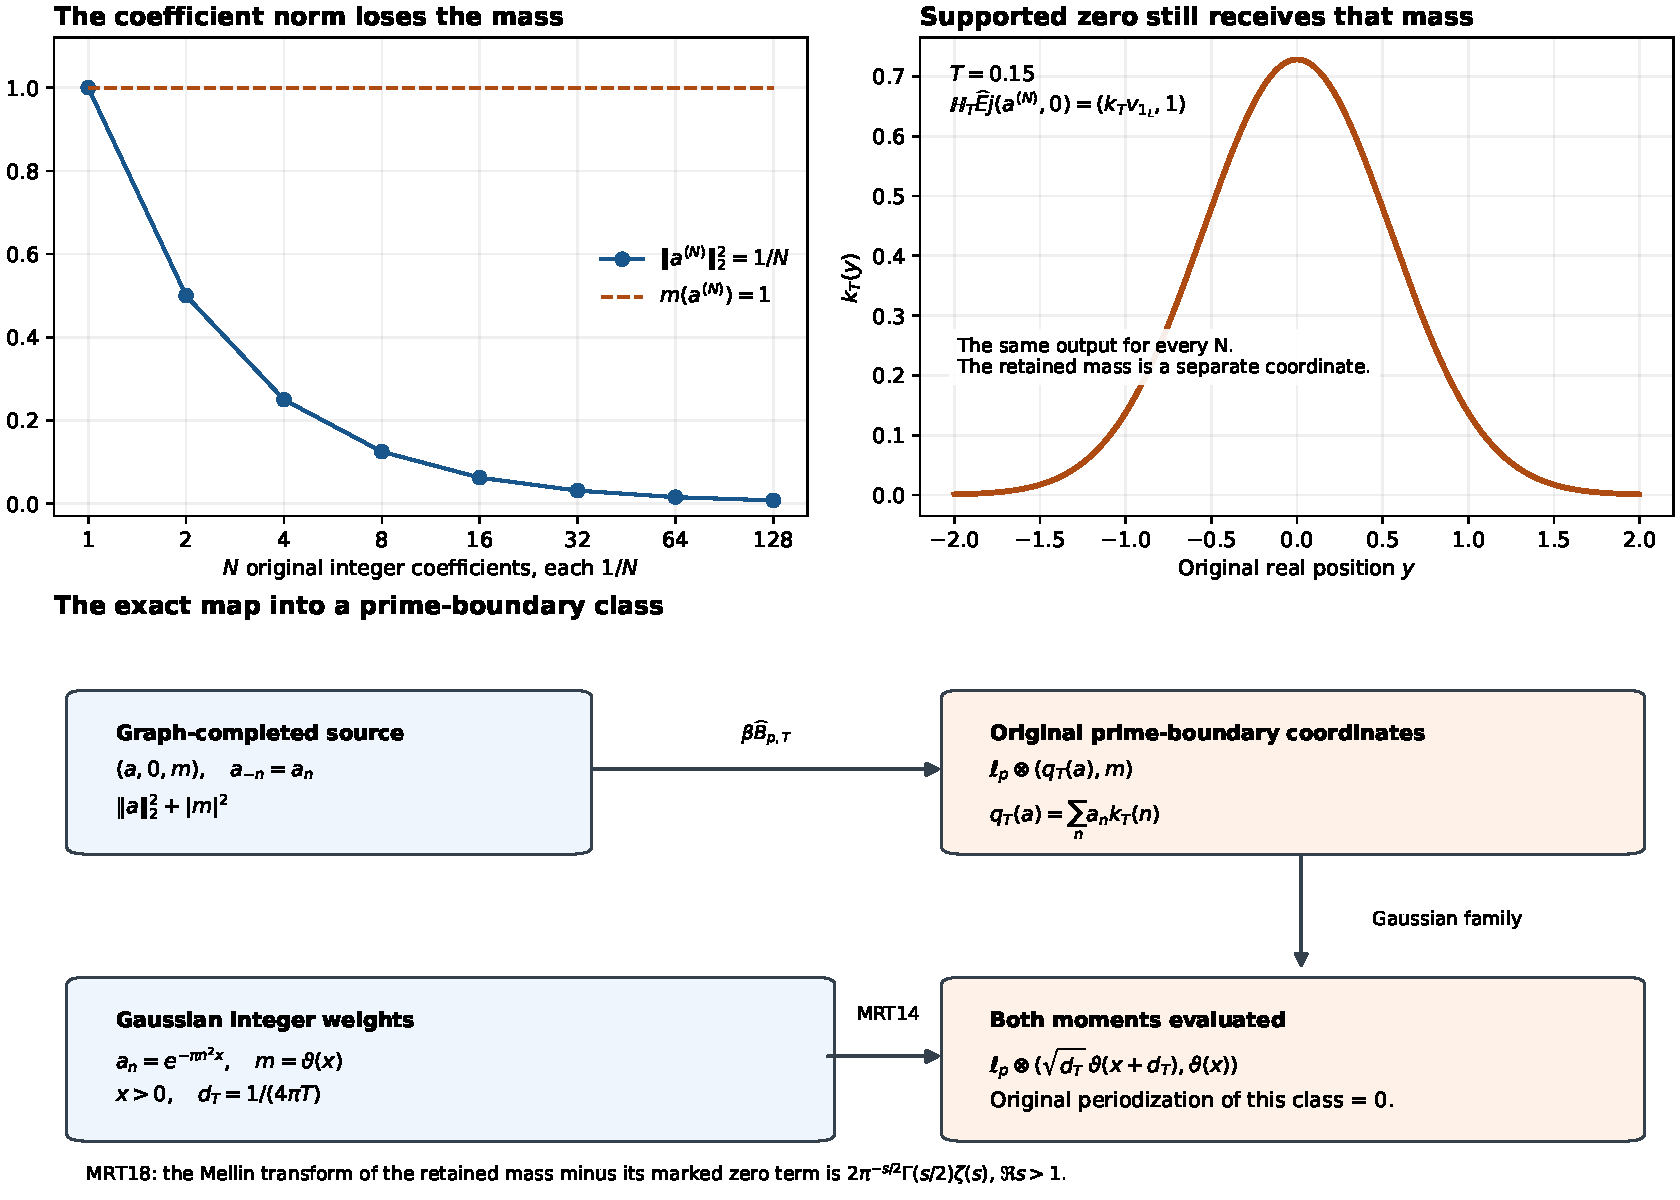
\includegraphics[width=\linewidth]{SUPPORTED_ZERO_MASS_RECEIVER.pdf}
\caption{Retaining the mass repairs the specified supported-zero
action. The left graph gives the exact coefficient norm of MCB3;
the right graph shows its identical supported-zero heat output,
at the stated time. The diagram records the actual prime-boundary
map MRT7--12, whose original periodization seminorm remains zero.
The Gaussian source MRT13--20 evaluates both boundary coordinates
and returns the original zeta function. Curves are numerical
renderings of the displayed exact formulas.}
\end{figure}
\section{The retained mass enters the actual prime-boundary receiver}
\label{sec:mass-theta-prime}

\paragraph{MRT1. The two source moments and their prime class.}
The preceding construction has an arithmetic receiver, which we
now calculate rather than identifying the two source spaces by
analogy. Use the even Schwartz space \(H=\mathcal S(\mathbb R)^{\rm even}\),
with the two original moments
\[
 m_H(h)=\left(h(0),\int_{\mathbb R}h(y)\,dy\right),\quad
 H_0=\ker m_H,\quad R=\mathbb C[\mathbb Q_{>0}^{\times}],\quad
 I=\ker(\operatorname{aug}:R\to\mathbb C).                 \tag{MRT1}
\]
The group basis elements obey \(t_at_b=t_{ab}\), without changing
the rational dilation parameter. The actual moment-zero source
and its algebraic coinvariants are
\[
 M_0=\ker(\operatorname{aug}\otimes m_H),\qquad
 Q_0=M_0/IM_0,\qquad
 \mathcal B=\bigoplus_{p\ {\rm prime}}\mathbb C\ell_p\otimes\mathbb C^2.
                                                               \tag{MRT2}
\]
These are the original periodization source and prime-boundary
coordinates of the published
\href{https://github.com/KokunoYumeto/zeta-function-research-reader/blob/ec73ac350d0cda3d95c0bd1361bede33166b4d34/workbenches/splitzero-tandem/continuations/20260923-original-zeta-return/NOTE.tex}{original-zeta return, FR15--25}.
The periodization and its measure come from
\href{https://arxiv.org/abs/math/9811068v1}{Alain Connes,
\emph{Trace formula in noncommutative geometry and the zeros of the
Riemann zeta function}}, Section III (6)--(19). The following
explicit coefficient map and its mass-completion extension are
derived here; they are not attributed to that article.

Here is the full algebra needed for this receiver. The functions
\[
 h_0(y)=(1-2\pi y^2)e^{-\pi y^2},\qquad
 h_1(y)=2\pi y^2e^{-\pi y^2}
\]
have moments \((1,0)\) and \((0,1)\), respectively. Gaussian
integration and evaluation prove these values. They give
\(H=H_0\oplus\operatorname{span}(h_0,h_1)\), so
\[
 Q_0\cong H_0\oplus(I/I^2)\otimes\mathbb C^2
       \cong H_0\oplus\mathcal B.                         \tag{MRT3}
\]
Indeed \(M_0=(R\otimes H_0)\oplus(I\otimes\mathbb C^2)\);
its multiplication by \(I\) has components
\(I\otimes H_0\) and \(I^2\otimes\mathbb C^2\).
In \(I/I^2\), the identity
\(t_{ab}-1=(t_a-1)+(t_b-1)+(t_a-1)(t_b-1)\), followed by
the prime factorization of a positive rational, expresses every
class as \(\sum_p v_p(a)[t_p-1]\). The linear functionals
\(t_a\mapsto v_p(a)\) kill \(I^2\) and separate these
generators. This proves both isomorphisms and their inverses.

Explicitly the coordinates of \(c=[\sum_a t_a\otimes h_a]\) are
\[
 \Phi c=\sum_a h_a,\qquad
 \beta(c)=\sum_p\ell_p\otimes\sum_a v_p(a)m_H(h_a).          \tag{MRT4}
\]
The defining source condition gives \(\Phi c\in H_0\).
An inverse to MRT3 sends \((h,\sum_p\ell_p\otimes u_p)\)
to
\[
 [1\otimes h]+\sum_p[(t_p-1)\otimes
                    (u_{p,0}h_0+u_{p,1}h_1)] .             \tag{MRT5}
\]
There are only finitely many nonzero \(u_p\). Changing the
moment lift changes this class by \(IM_0\). These calculations
verify all quotient relations; the receiver is not merely a
map on arbitrarily selected representatives.

\paragraph{MRT2. The heat coefficient source has an exact two-moment map.}
Take an even finitely supported coefficient sequence \(a\), with
\(a_{-n}=a_n\), no lower coefficients for this specified arrow,
and the unchanged \(T>0\). Its heat function \(h=A_Ta\) of
MCB12 belongs to \(H\). Direct evaluation and integration give
\[
 q_T(a)=\sum_n a_n k_T(n),\qquad m(a)=\sum_n a_n,\qquad
 m_H(A_Ta)=(q_T(a),m(a)).                                  \tag{MRT6}
\]
Consequently, for every original arithmetic prime \(p\), the map
\[
 B_{p,T}(a)=[(t_p-1)\otimes A_Ta]\in Q_0
\]
has the exact coordinates
\[
 (\Phi,\beta)B_{p,T}(a)
        =(0,\ell_p\otimes(q_T(a),m(a))).                   \tag{MRT7}
\]
The first zero follows by subtraction of the same function, and
the second follows from \(v_p(p)=1\), \(v_p(1)=0\).
This is the connecting map from the actual integer heat source
to the existing prime-boundary source.

Write \(k_0=k_T(0)\), \(k_1=k_T(1)\); these symbols retain
the values \((4\pi T)^{-1/2}\) and
\((4\pi T)^{-1/2}e^{-1/(4T)}\). For any pair \((u_0,u_1)\),
put
\[
 a_0=\frac{u_0-k_1u_1}{k_0-k_1},\qquad
 a_{1}=a_{-1}=\frac{k_0u_1-u_0}{2(k_0-k_1)},\qquad
 a_n=0\quad(|n|>1).                                      \tag{MRT8}
\]
Since \(k_0>k_1\), this is defined. Substitution gives
\(q_T(a)=u_0\) and \(m(a)=u_1\). Thus this actual finite
source attains both prime-boundary moments, with their original
coefficients and Gaussian constants. It is not confined to a
single prescribed moment ratio.

\paragraph{MRT3. Completion and supported-zero action commute with this map.}
Let \(\widehat V_E^{\rm even,top}\) be the closed subspace
\((a,0,m)\) of MCB5 with even \(a\). The samples
\((k_T(n))_n\) lie in \(\ell^2\); hence Cauchy--Schwarz gives
\[
 |q_T(a)|\le
 \left(\sum_n k_T(n)^2\right)^{1/2}\|a\|_2.              \tag{MRT9}
\]
The same formula with an independent last coordinate extends MRT7:
\[
 \widehat B_{p,T}(a,0,m)=
 b\bigl(\ell_p\otimes(q_T(a),m)\bigr),                   \tag{MRT10}
\]
where \(b\) is the explicit map MRT5 on its second summand.
The two scalar coordinates are continuous in the literal graph
norm. No new norm is assigned to the adelic quotient in this
statement. Even finite graph sources are dense in this subspace:
in MCB6 choose the correcting sets in opposite pairs, retaining
the same total correction and its vanishing squared norm.

The original supported-zero operator now has the following
arithmetic receiving matrix, with all constants retained:
\[
 J_T=\begin{pmatrix}0&k_T(0)\\0&1\end{pmatrix},\qquad
 J_T^2=J_T,\qquad
 \widehat B_{p,T}\widehat E
   =b\,(\operatorname{id}_{\mathbb C\ell_p}\otimes J_T)
                         \beta\widehat B_{p,T}.            \tag{MRT11}
\]
Indeed \(\widehat E(a,0,m)=(m\delta_0,0,m)\), whose two
moments are \((k_T(0)m,m)\). This proves MRT11 exactly;
it does not assert a not-yet-defined multiplication on all of
\(Q_0\). On the completed pure-mass vector \((0,0,1)\),
MRT10 gives \(b(\ell_p\otimes(0,1))\); after \(\widehat E\)
it gives \(b(\ell_p\otimes(k_T(0),1))\). The boundary action
is consequently visible in the actual two-moment coordinates.

\paragraph{MRT4. Relation to the original periodization seminorm.}
Keep exactly the original periodization and its measure:
\[
 \mathcal E(c)(x)=x^{1/2}\,2\sum_{n\ge1}(\Phi c)(nx),\qquad
 \|c\|_\delta^2=\int_0^\infty|\mathcal E(c)(x)|^2
                 (1+\log^2x)^{\delta/2}\frac{dx}{x},
 \quad\delta>1.                                          \tag{MRT12}
\]
Connes's compact-unit measure has mass one in this formula; with
mass \(c_K\) the whole displayed integral has the factor \(c_K\),
which is retained. For every vector in MRT10, \(\Phi=0\),
so \(\mathcal E=0\) and this exact seminorm is zero. Whenever
\((q_T(a),m)\ne(0,0)\), MRT3 proves that its boundary class is
nonzero. This verifies on the actual Gaussian coefficient source
the failure of its two moments to descend through the Hausdorff
quotient of MRT12. The graph completion MCB5 repairs the domain
of supported-zero multiplication; it does not turn MRT12 into
a positive norm on these prime classes. The maps MRT7--12 retain
both facts and give their exact connection.

\paragraph{MRT5. The theta family is an admitted source, with two evaluated moments.}
Let \(x>0\), independently of the heat time \(T\), and put
\[
 a^{x}_n=e^{-\pi n^2x},\qquad
 \vartheta(x)=\sum_{n\in\mathbb Z}e^{-\pi n^2x},\qquad
 d_T=\frac1{4\pi T},\qquad k_T(0)=\sqrt{d_T}.             \tag{MRT13}
\]
These original weights are even and absolutely summable. Their
finite truncations converge in the graph norm to
\((a^x,0,\vartheta(x))\): both the squared tails and the mass
tails tend to zero by Gaussian convergence. Unlike the unweighted
integer comb, this is an admitted vector of MCB5.

Moreover \(A_Ta^x\) is an even Schwartz function. To see every
Schwartz bound directly, each derivative of \(k_T(y-n)\) is a
fixed polynomial in \(y-n\) times its Gaussian. For any integer
\(M\ge0\), use
\(1+|y|\le(1+|n|)(1+|y-n|)\). The supremum of the resulting
polynomial times that Gaussian is finite, and its sum against
\((1+|n|)^M e^{-\pi n^2x}\) is finite. Uniform derivative
convergence proves the assertion. Hence MRT7 applies directly
to this actual Schwartz function, not just to its completed image.
Evaluation and integration in MRT6 yield
\[
 \beta B_{p,T}(a^x)=
 \ell_p\otimes\left(
    \sqrt{d_T}\,\vartheta(x+d_T),\ \vartheta(x)\right).
                                                               \tag{MRT14}
\]
The product of the two Gaussian factors proves the first entry,
and integration of each translate proves the second. After the
supported-zero action the same class has moments
\[
 \ell_p\otimes\left(
     \sqrt{d_T}\,\vartheta(x),\ \vartheta(x)\right).       \tag{MRT15}
\]
Thus the change in this prime-boundary coordinate, in the order
before minus after, is exactly
\[
 \ell_p\otimes\left(
   \sqrt{d_T}[\vartheta(x+d_T)-\vartheta(x)],\ 0\right).
                                                               \tag{MRT16}
\]
It is nonzero for every \(x,T>0\), since every pair of nonzero
integer Gaussian terms strictly decreases when its parameter
increases by \(d_T>0\). This evaluates an actual arithmetic
consequence of the supported-zero operation in the retained source.

\paragraph{MRT6. Return to the original zeta function, with the marked term kept.}
The single integer-zero source is \(\delta_0\), with coefficient
one, mass one and heat moments \((\sqrt{d_T},1)\). Keep it
as a separate summand. The remaining pair from MRT14 is
\[
 \left(\sqrt{d_T}[\vartheta(x+d_T)-1],\ \vartheta(x)-1\right).
                                                               \tag{MRT17}
\]
For \(\Re s>1\), its second Mellin integral is exactly
\[
 \int_0^\infty[\vartheta(x)-1]x^{s/2-1}dx
   =2\pi^{-s/2}\Gamma(s/2)\zeta(s),\qquad
 \zeta(s)=\frac{\pi^{s/2}}{2\Gamma(s/2)}
                \int_0^\infty[\vartheta(x)-1]x^{s/2-1}dx.
                                                               \tag{MRT18}
\]
Indeed the paired integers \(\pm n\) give the factor two;
the substitution \(y=\pi n^2x\) gives
\(\pi^{-s/2}n^{-s}\Gamma(s/2)\); absolute interchange follows
from \(\sum n^{-\Re s}<\infty\). The marked constant has
no Mellin convergence half-plane on \((0,\infty)\) and remains
separate, rather than being assigned zero. Poisson reflection and
splitting at one retain two distinct endpoint contributions: the
zero source coefficient gives \(-1/s\), and the zero Fourier
coefficient gives \(1/(s-1)\), as derived in LH15. Thus original \(\zeta\)
and all its continuation factors remain explicit.

The first coordinate also has an evaluated Mellin transform:
for \(\Re s>0\),
\[
 \int_0^\infty\sqrt{d_T}[\vartheta(x+d_T)-1]x^{s/2-1}dx
  =2\sqrt{d_T}\,\pi^{-s/2}\Gamma(s/2)
         \sum_{n\ge1}e^{-\pi d_Tn^2}n^{-s}.                \tag{MRT19}
\]
Here the same calculation is absolutely convergent already for
\(\Re s>0\), because the Gaussian coefficient controls the
integer sum. The full Dirichlet series in MRT19 is entire in
\(s\), by uniform Gaussian convergence on compact sets; the
Gamma factor is retained. In the common half-plane \(\Re s>1\),
the Mellin transform of MRT16 is therefore
\[
 2\sqrt{d_T}\,\pi^{-s/2}\Gamma(s/2)
       \left[\sum_{n\ge1}e^{-\pi d_Tn^2}n^{-s}-\zeta(s)\right]
       \ell_p\otimes(1,0).                               \tag{MRT20}
\]
Every term in this difference has now been identified. In particular
the zero-seminorm prime-boundary source contains a family whose
retained mass returns the original zeta function. This is a proved
receiver and a proved loss of specified data under MRT12; it is
not an evaluation of the full Weil pairing on a newly invented norm.

\section{The endpoint obstruction defines a two-dimensional heat boundary}
\label{sec:endpoint-sectorial-heat}

\paragraph{ESH1. The original theta density before its differential filter.}
Keep the original coordinate \(s=\tfrac12+\tfrac{iZ}{2}\), and
the full factor \(A(s)=\pi^{-s/2}\Gamma(s/2)\). The theta
formula LH15, with the exact substitution \(x=e^{4u}\), gives
\[
 A(s)\zeta(s)=\int_0^\infty\rho(u)\cos(Zu)\,du,\qquad
 \rho(u)=8e^u\psi(e^{4u})-4e^{-u},\qquad |\Im Z|<1.
                                                               \tag{ESH1}
\]
Indeed the two integral terms in LH15 become
\(8\int_0^\infty e^u\psi(e^{4u})\cos(Zu)du\).
Its rational endpoint contribution is
\(1/[s(s-1)]=-4/(1+Z^2)\), equal to the retained
\(-4e^{-u}\) integral on the stated strip. Both endpoint
terms are consequently present in ESH1. The density and the
subsequent theta filter use the original definitions of
\href{https://arxiv.org/abs/1801.05914v5}{Brad Rodgers and
Terence Tao, \emph{The de Bruijn--Newman constant is non-negative}},
equations \texttt{phidef}, \texttt{htdef}, \texttt{hoz} and
\texttt{sas}; the unfiltered sectorial extension is derived here.

The original unfiltered real-axis integral after inserting a
heat weight is
\[
 I_t(Z)=\int_0^\infty e^{tu^2}\rho(u)\cos(Zu)\,du.
                                                               \tag{ESH2}
\]
It converges for \(\Re t<0\), for every complex \(Z\),
locally uniformly together with all derivatives. The part
\(8e^u\psi(e^{4u})\) has faster than Gaussian decay, while
the endpoint part has Gaussian decay precisely in this left
half-plane. For positive real \(t\) and \(Z=0\), the latter
part diverges with one sign. Thus the original real-axis formula
does not define an entire-in-\(Z\) heat family at positive time.
An analytic continuation must be specified rather than calling
that same improper integral convergent.

\paragraph{ESH2. Exact lateral continuations of the endpoint.}
Set \(q=-t\), first \(q>0\). For any complex \(a\),
completing the square gives
\[
 F(q,a)=\int_0^\infty e^{-qu^2-au}du
 =\frac{\sqrt\pi}{2\sqrt q}
       e^{a^2/(4q)}\operatorname{erfc}\!\left(\frac a{2\sqrt q}\right).
                                                               \tag{ESH3}
\]
For real \(a\) this is a direct real integral substitution;
both sides are entire in \(a\) by Gaussian domination and
the entire power series of \(\operatorname{erfc}\), so the
identity holds for all \(a\). The right side extends analytically
to \(q\in\mathbb C\setminus(-\infty,0]\), with the square
root positive on the positive real axis. This specifies the branch.
Here
\(\operatorname{erfc}(z)=1-\frac2{\sqrt\pi}\int_0^z e^{-v^2}dv\);
its entire primitive immediately proves
\(\operatorname{erfc}(z)+\operatorname{erfc}(-z)=2\).
This is the convention of N. M. Temme,
\href{https://dlmf.nist.gov/7.2.E2}{NIST DLMF, equation 7.2.2};
the original equation TeX is retained with the source record.

The endpoint cosine integral is
\[
 B(q,Z)=\tfrac12\{F(q,1-iZ)+F(q,1+iZ)\}.                 \tag{ESH4}
\]
For positive real \(t\), define \(B_+(t,Z)\) and
\(B_-(t,Z)\) by approaching \(q=-t\) from the upper and
lower \(q\)-half-planes, respectively. The square roots are
\(+i\sqrt t\) and \(-i\sqrt t\). Thus ESH3 and the
displayed erfc identity give the exact difference
\[
 F_+(t,a)-F_-(t,a)
       =-i\sqrt{\frac\pi t}\,e^{-a^2/(4t)},
\quad
 B_+(t,Z)-B_-(t,Z)
       =-i\sqrt{\frac\pi t}\,
          e^{(Z^2-1)/(4t)}\cos\!\frac Z{2t}.              \tag{ESH5}
\]
This orientation uses the \(q\)-plane; reversing the order of
the two lateral values reverses the sign.

The rapidly decaying part
\[
 L_t(Z)=8\int_0^\infty e^{tu^2+u}\psi(e^{4u})\cos(Zu)du
\]
is jointly entire in \((t,Z)\). The two unfiltered continuations
at positive time are therefore
\[
 I_\pm(t,Z)=L_t(Z)-4B_\pm(t,Z),\qquad
 I_+-I_-=4i\sqrt{\frac\pi t}\,
                 e^{(Z^2-1)/(4t)}\cos\!\frac Z{2t}.
                                                               \tag{ESH6}
\]
The factor four and its sign come from the original endpoint
density in ESH1. Each branch satisfies
\(\partial_t I=-\partial_Z^2 I\): differentiate the integral
in \(\Re t<0\), then use analytic continuation on its
specified branch. This continuation assertion does not make
ESH2 converge at positive real time.

\paragraph{ESH3. The full theta filter and its exact kernel.}
Define, without suppressing its time-dependent terms,
\[
 \mathcal N_t=-\frac{1+(Z-2t\partial_Z)^2}{64}
 =-\frac{1+Z^2-2t-4tZ\partial_Z+4t^2\partial_Z^2}{64}.
                                                               \tag{ESH7}
\]
For a twice differentiable density with the decay of \(\rho\),
two integrations by parts in \(\Re t<0\) give
\[
 \int_0^\infty e^{tu^2}\rho''(u)\cos(Zu)du
  =-\rho'(0)-(Z-2t\partial_Z)^2 I_t(Z).                  \tag{ESH8}
\]
The first boundary at infinity vanishes; at zero it is
\(-\rho'(0)\). The second boundary is zero because the
derivative of \(e^{tu^2}\cos(Zu)\) vanishes at zero.
Differentiating that whole weight twice gives precisely
\((2t+4t^2u^2-Z^2)\cos(Zu)-4tZu\sin(Zu)\),
which verifies every term of ESH8.

The Poisson identity in LH14 yields
\(\psi'(1)=-\psi(1)/4-1/8\). Consequently
\[
 \rho'(0)=8\psi(1)+32\psi'(1)+4=0.                     \tag{ESH9}
\]
There has been no dropped endpoint boundary. Direct differentiation
of the entire density, with \(x=e^{4u}\), gives
\[
 \frac{\rho''(u)-\rho(u)}{64}
 =\sum_{n\ge1}
   \left(2\pi^2n^4e^{9u}-3\pi n^2e^{5u}\right)e^{-\pi n^2e^{4u}}
 =\Phi(u).                                               \tag{ESH10}
\]
The \(-4e^{-u}\) term is annihilated by \(\partial_u^2-1\),
but its boundary contribution has already been included in ESH9.
ESH8--10 prove, first in \(\Re t<0\) and then along each
continuation, the exact identity
\[
 \mathcal N_t I_+(t,Z)=\mathcal N_t I_-(t,Z)
        =H_t(Z)=\int_0^\infty e^{tu^2}\Phi(u)\cos(Zu)du.
                                                               \tag{ESH11}
\]
The integral for \(H_t\) is jointly entire by the decay of
\(\Phi\). This is a derived equality between the two specified
heat constructions, including their lost boundary directions.
The two density parts separately have nonzero boundary terms:
\[
 \mathcal N_t B=-\frac1{64},\qquad
 \mathcal N_t L_t=H_t-\frac1{16},\qquad
 \mathcal N_t(L_t-4B)=H_t.                              \tag{ESH17}
\]
For the first equation the endpoint density satisfies
\(\rho''=\rho\), \(\rho'(0)=-1\), so ESH8 gives it
directly. For the second, the theta-only density has derivative
\(-4\) at zero by ESH9 and the endpoint derivative \(+4\)
in the full density. Its interior filtered density is still
\(\Phi\). Substitution in ESH8 yields the displayed
\(-1/16\), which the endpoint contribution cancels exactly.
Thus annihilating the interior endpoint density does not authorize
omitting its integration boundary.

For each \(t\ne0\), the kernel of \(\mathcal N_t\) on the
entire functions of \(Z\) is exactly
\[
 \left\{
 e^{Z^2/(4t)}
 \left(c_+e^{iZ/(2t)}+c_-e^{-iZ/(2t)}\right):
          c_+,c_-\in\mathbb C\right\}.                   \tag{ESH12}
\]
To prove completeness of this list, write
\(f=e^{Z^2/(4t)}g\). Then
\((Z-2t\partial_Z)f=-2t e^{Z^2/(4t)}g'\), and the
kernel equation becomes \(g+4t^2g''=0\). Its two initial
values determine its entire solution by the coefficient recursion,
giving exactly the two displayed exponentials. ESH5 lies in this
space, so its annihilation in ESH11 is also verified directly.
The actual cosine source is even in \(Z\). On this original
even domain the kernel is one-dimensional: evenness in ESH12
requires \(c_+=c_-\), leaving
\(e^{Z^2/(4t)}\cos(Z/(2t))\). The sine direction belongs
to the explicitly larger, nonsymmetric entire-function domain.
Thus the actual lateral jump occupies exactly the symmetric
kernel direction, not two independently varied cosine parameters.
The time dependence of any such homogeneous difference which
also satisfies the heat equation is determined. Writing the
two coefficients in ESH12 as functions \(c_\pm(t)\), direct
differentiation gives
\[
 c_\pm'(t)+\left(\frac1{2t}-\frac1{4t^2}\right)c_\pm(t)=0,
 \qquad c_\pm(t)=C_\pm t^{-1/2}e^{-1/(4t)}.              \tag{ESH18}
\]
On a fixed simply connected time domain avoiding zero the chosen
square root makes this formula single-valued. The two independent
space exponentials force both scalar equations, and integrating
them gives exactly the stated constants. In original \(s\)
coordinates the modes are \(t^{-1/2}e^{-s^2/t}\) and
\(t^{-1/2}e^{-(s-1)^2/t}\). The even source requires equal
coefficients, recovering the time dependence of ESH6 and ESH14.

\paragraph{ESH4. Both original-zeta receivers and the endpoint modes.}
Return to the original coordinate \(Z=-2i(s-1/2)\) and keep
\[
 f_\pm(t,s)=\frac{I_\pm(t,-2i(s-1/2))}
                   {\pi^{-s/2}\Gamma(s/2)},\qquad
 z_t(s)=\frac{16H_t(-2i(s-1/2))}
                 {s(s-1)\pi^{-s/2}\Gamma(s/2)}.           \tag{ESH13}
\]
The first family is defined on the sectorial branches just proved;
the second is CF1's returned meromorphic family. Both recover the
original \(\zeta(s)\) at time zero on \(0<\Re s<1\):
for the first, approach zero through \(t<0\) and dominate the
endpoint integral by \(e^{-(1-|\Im Z|)u}\); for the second,
use ESH1 and \(16\mathcal N_0=s(s-1)\).
Their domains at time zero and their later poles have not been
identified merely from their common initial values.

The actual two endpoint modes in the original coordinate are
\(e^{-s^2/t}\) and \(e^{-(s-1)^2/t}\). Specifically,
\[
 f_+(t,s)-f_-(t,s)
  =2i\sqrt{\frac\pi t}\,
       \frac{\pi^{s/2}}{\Gamma(s/2)}
          \left[e^{-s^2/t}+e^{-(s-1)^2/t}\right].          \tag{ESH14}
\]
This follows by expanding the cosine in ESH6 and substituting
the stated coordinate, with no rescaling of time.

The complete differential receiving map is
\[
 z_t(s)=\frac{
  [s(s-1)+t/2]A(s)f_\pm(t,s)
   +\frac{t(2s-1)}2\partial_s[A(s)f_\pm(t,s)]
   +\frac{t^2}4\partial_s^2[A(s)f_\pm(t,s)]
 }{s(s-1)A(s)}.                                         \tag{ESH15}
\]
For verification, \(Z-2t\partial_Z=-i[(2s-1)+t\partial_s]\);
squaring retains the extra derivative term \(2t\).
Multiplication by 16 in ESH7 then gives exactly the numerator
of ESH15. This proves the equality away from the displayed
exceptional factors and hence meromorphically, with the original
factor germs retained. The first derivative contributes
\(A'f+Af'\), and the second contributes
\(A''f+2A'f'+Af''\), with
\[
 A'/A=-\tfrac12\log\pi+\tfrac12\psi_{\Gamma}(s/2),\qquad
 A''/A=\tfrac14\psi_{\Gamma}'(s/2)
       +[-\tfrac12\log\pi+\tfrac12\psi_{\Gamma}(s/2)]^2.
                                                               \tag{ESH16}
\]
Here \(\psi_{\Gamma}\) denotes the Gamma logarithmic derivative,
distinct from the theta sum \(\psi(x)\). Every derivative of
the original multiplier is therefore specified.

At fixed \(t\ne0\) on these branches, \(I_\pm\) is entire
in \(s\), as is \(1/A(s)\), so \(f_\pm\) is entire. In
contrast, CF27 proves that \(z_t\) has a nonzero pole at one
for real \(t\). ESH15 is the exact map between these different
analytic domains; its denominator and derivatives cannot be
deleted. The recovery of \(\zeta\)'s pole as \(t\to0\) for
the sectorial family is not locally uniform at that pole, since
a locally uniform limit of holomorphic functions would be
holomorphic there. This identifies the precise endpoint domain
change, not a failure of the proved convergence in the open strip.

Thus the obstruction ESH2 defines both a two-branch continuation
and the explicit two-dimensional entire kernel ESH12, whose
intersection with the actual even source is one-dimensional.
The map to the theta heat family annihilates exactly these
homogeneous directions on the respective stated domains at each
nonzero time. Keeping a chosen continued
source and its endpoint coordinates preserves them; the
subsequent map to the original \(\zeta\) is ESH13--16 with
all factors retained. No conclusion about RH follows merely
from forgetting or retaining this computed kernel.

\end{document}
